\documentclass[a4paper,11pt,twoside,openany]{book}

\usepackage{tipx}
\usepackage{algo}
% \usepackage[named]{libtex/algo}
\usepackage{algorithm}
\usepackage[noend]{algpseudocode}
\usepackage{amssymb}
\usepackage{amsthm}
\setcounter{tocdepth}{3}
\usepackage{graphicx}
\usepackage{amsfonts}
\usepackage{epsfig}
\usepackage{multirow}
\usepackage{amsfonts,amsmath}
\usepackage{srcltx}
\usepackage{multirow}
\usepackage{dsfont}
\usepackage{booktabs}
\usepackage[countmax]{subfloat}
\usepackage{subcaption}
\usepackage{color}
\usepackage[table]{xcolor}
\usepackage{tabularx}
\usepackage{subfig}
\usepackage{url}
\usepackage{makeidx}
\usepackage{graphicx}
\usepackage{libtex/thesisStyle}
\usepackage{float}


%%%%%%%%%%%%%
\long\def\comment#1{}


\newlength{\figtblfootnotemargin}
\newlength{\figtblfootnotewidth}

\setlength{\figtblfootnotemargin}{15mm}
\setlength{\figtblfootnotewidth}{\textwidth}
\addtolength{\figtblfootnotewidth}{-\figtblfootnotemargin}


%---------------------------------

\newcommand{\db}[1]{
    {\tt #1}
}

%---------------------------------
\newcommand{\outcomment}[1]{
    %\comment{
    \begin{quote}
       {\scriptsize
       {\em OC:} #1
%        #1
       }
    \end{quote}
    %}
}

%---------------------------------

\newcommand{\myheader}[1]{
    \godown
    $\bullet$ {\bf #1} \nn
}

%---------------------------------

\newcommand{\SquareOfSize}[2]{
 \fbox{\hsize #1cm \hbox to #1cm{\vbox{#2}}}
}

\newcommand{\figSquare}[1]{
   \hfill
        \SquareOfSize{13}
            { \vparag \vparag #1 \vparag \vparag }
    \hfill
}

\newcommand{\figSquareLarge}[1]{
   \hfill
        \SquareOfSize{16}
            { \vparag \vparag #1 \parag \vparag }
    \hfill
}

\newcommand{\SQUARE}[1]{
        \SquareOfSize{15}{#1}
}

\newcommand{\SquareSlite}[1]{
        \SquareOfSize{16}{#1}
}


\newcommand{\Syntax}[2]{ ``#1'', where #2 }

\newcommand{\SYNTAX}[2]{
    \SquareOfSize{14}{ \small
        #1 \hfill #2
    }
}

\newcommand{\UpdateProcess}[1]{
    \SquareOfSize{14}{  \bf
        #1
    }
}


\newcommand{\mathdef}[1]
{
    {\small
    \bq {\em Definition.}
        #1
    \eq
    }
}

\newcommand{\pqiCom}[2]{
    \parbox[t]{2cm}{#1} \ \parbox[t]{13.5cm}{ #2}
}

\newcommand{\KEYPOINT}[2]{
\SQUARE{\parbox[t]{3cm}{\small \em  #1} \ \parbox[t]{10cm}{{\bf #2}}}}

%\newcommand{\KEYPOINT}[2]{
%\SQUARE{\small \em  #1: \ \ \parbox[t]{10cm}{{\bf #2}}}}

%___________________________________________________________
\newcommand{\conclusion}[3]{
 \bc
    $ \left.  \begin{array}{r}
                    #1 \\
                    #2
                \end{array}
                    \right\}  \rightarrow #3
            $
 \ec
}
%___________________________________________________________

%-------- Update Operations --------------

\newcommand{\BriefDescription}{$\bullet$
    {\em ������� ���������:} \\}

\newcommand{\CheckedConstraint}
   {$\bullet$ {\em ���������� ������� ����������� :} \\}

\newcommand{\ExecutionAnalysis}[1]{
    $\bullet$ {\em ��������� ��������� :} \\
    \parbox[t]{2cm}{\hspace{2cm}} \ \parbox[t]{12cm}{ {\small #1} }
}

\newcommand{\SemanticAnalysis}[1]{
    $\bullet$ {\em ������������ �������������� ��������� :} \\
    \parbox[t]{2cm}{\hspace{2cm}} \ \parbox[t]{12cm}{ {\small #1} }
}

\newcommand{\namecheck}{ ������� ��������� ���� ������������ }

%--------  ---------------- --------------

\newcommand{\EFupdate}[3]{
    \item  {\scriptsize �����}: #1 {\scriptsize ��������} : $#2$

    \hspace*{1cm} \parbox[t]{12cm}{#3}
}

\newcommand{\visiblecomment}[1]{
  \underline{\centerline{ \bf ������}}\\
     \vspace{0.3cm}
     \bc
      \parbox[t]{14cm}{
            \small \em #1
      } \\
    \ec
  \underline{\centerline{ \bf ����� �������}}
}

\newcommand{\slidefigure}[3]{
% \slidefigure{#1 figure_text}
%             {#2 figure_name}
%             {#3 height_in_mm}

    \begin{figure}[ht]
                    \comment{\rule[0.2in]{\textwidth}{.01in}}
        {\Large \mbox{#1}}
        \centerline{
            \psfig{figure=#2,height=#3}
        }
    \end{figure}
}



\newcommand{\putsinglefigureR}[2]{
% \putsinglefigure{#1 figure_name}
%                 {#2 height_in_mm}

    \begin{figure}[htbp]
        \psfig{figure=#1,height=#2}
    \end{figure}
}

\newcommand{\putsinglefigure}[2]{
% \putsinglefigure{#1 figure_name}
%                 {#2 height_in_mm}

%   \begin{figure}[htbp]            <- not supported in landscape !
        \centerline{
        \psfig{figure=#1,height=#2}
        }
%   \end{figure}
}

\newcommand{\putsfigure}[2]{
        \psfig{figure=#1,height=#2}
}

\newcommand{\putfigure}[5]{
% \putfigure{#1 figure_name}
%           {#2 height_in_mm}
%           {#3 figure_label}
%           {#4 figure_title}
%           {#5 figure_text}

    \begin{figure}[htbp]
        \centerline{ \psfig{figure=#1,height=#2}}
        %\vspace*{-0.3cm} % added 4/5/2001 for EJM conf
        \caption{#4}{\vspace*{0.01cm}  \centerline{ \parbox[t]{13cm}{\footnotesize #5}}}
        \label{#3}
        %\vspace*{-0.6cm} % added 4/5/2001 for EJM conf
    \end{figure}
}



\newcommand{\putfigureVLDB}[5]{
% \putfigure{#1 figure_name}
%           {#2 height_in_mm}
%           {#3 figure_label}
%           {#4 figure_title}
%           {#5 figure_text}

    \begin{figure}[htbp]
        \centerline{ \psfig{figure=#1,height=#2}}
        \vspace*{-0.3cm} % added 4/5/2001 for EJM conf
        \caption{#4}{\vspace*{0.01cm}  \centerline{ \parbox[t]{9cm}{\footnotesize #5}}}
        \label{#3}
        \vspace*{-0.6cm} % added 4/5/2001 for EJM conf
    \end{figure}
}


\newcommand{\putfigureSV}[5]{
% \putfigurSVe{#1 figure_name}  SV = for Springer-Verlag
%           {#2 height_in_mm}
%           {#3 figure_label}
%           {#4 figure_title}
%           {#5 figure_text}

    \begin{figure}[htbp]
        \vspace*{-0.2cm}
        %\vspace*{-0.4cm}
        \centerline{ \psfig{figure=#1,height=#2}}
        \vspace*{-0.3cm}
        \caption{#4}{\vspace*{0.02cm}  \centerline{ \parbox[t]{10cm}{ #5}}}
        \label{#3}
        \vspace*{-0.8cm}
    \end{figure}
}


\newcommand{\putgeneralfigureNEW}[4]{
%           {#1 figure body}
%           {#2 figure_label}
%           {#3 figure_title}
%           {#4 figure_text}
    \begin{figure}[htbp]
        #1
        \vspace*{-0.5cm} % added 4/5/2001 for EJM conf
        \caption{#3}{\vspace*{0.001cm} \centerline{ \parbox[t]{13cm}{\footnotesize #4}}}
        %\caption{#3}{\vspace*{0.1cm} \centerline{ \parbox[t]{\textwidth}{\footnotesize #4}}}
        \label{#2}
        \vspace*{-0.4cm} % added 4/5/2001 for EJM conf
    \end{figure}
}

\newcommand{\putgeneralfigure}[4]{
%           {#1 figure body}
%           {#2 figure_label}
%           {#3 figure_title}
%           {#4 figure_text}

    \begin{figure}[htbp]
        #1
        \vspace*{-0.5cm} % added 4/5/2001 for EJM conf
        \caption{#3}{\vspace*{0.001cm} \centerline{ \parbox[t]{13cm}{\footnotesize #4}}}
        %\caption{#3}{\vspace*{0.1cm} \centerline{ \parbox[t]{\textwidth}{\footnotesize #4}}}
        \label{#2}
        \vspace*{-0.4cm} % added 4/5/2001 for EJM conf
    \end{figure}
}


\newcommand{\putTwoFiguresEngl}[6]{
    \begin{center}
    \begin{figure}
        \begin{minipage}[b]{0.5\textwidth}  %{7cm}
            \centerline{\putsfigure{#1}{#3}}
            \vspace*{3mm} \centerline{(a)}
        \end{minipage}
        \hspace*{0.5cm}
        \begin{minipage}[b]{0.5\textwidth}  %{7cm}
            \centerline{\putsfigure{#2}{#3}}
            \vspace*{3mm} \centerline{(b)}
        \end{minipage}
        \caption{#5}{\vspace*{0.1cm}
            \centerline{ \parbox[t]{13cm}{\footnotesize #6}}}
        \label{#4}
        \vspace*{-5mm} % added 15/9/2004
    \end{figure}
    \end{center}
}



\newcommand{\putTwoFiguresEnglSquare}[6]{
    %\begin{center}
    \begin{figure}
        \begin{minipage}[b]{85mm}
            \centerline{\fbox{\putsfigure{#1}{#3}}}
            \vspace*{3mm} \centerline{(a)}
        \end{minipage}
        \begin{minipage}[b]{85mm}
            \centerline{\fbox{\putsfigure{#2}{#3}}}
            \vspace*{3mm} \centerline{(b)}
        \end{minipage}
        \vspace*{-0.3cm}
        \caption{#5}{\vspace*{0.1cm}
            \centerline{ \parbox[t]{13cm}{\footnotesize #6}}}
        \label{#4}
        \vspace*{-8mm} % added 15/9/2004
    \end{figure}
    %\end{center}
}

\newcommand{\putFourFiguresEnglSquare}[8]{
    %\begin{center}
    \begin{figure}
        \begin{minipage}[b]{40mm}
            \centerline{\fbox{\putsfigure{#1}{#5}}}
            \vspace*{3mm} \centerline{(a)}
        \end{minipage}
        \begin{minipage}[b]{40mm}
            \centerline{\fbox{\putsfigure{#2}{#5}}}
            \vspace*{3mm} \centerline{(b)}
        \end{minipage}
        \begin{minipage}[b]{40mm}
            \centerline{\fbox{\putsfigure{#3}{#5}}}
            \vspace*{3mm} \centerline{(c)}
        \end{minipage}

        \begin{minipage}[b]{40mm}
            \centerline{\fbox{\putsfigure{#4}{#5}}}
            \vspace*{3mm} \centerline{(d)}
        \end{minipage}
        \caption{#7}{\vspace*{0.1cm}
            \centerline{ \parbox[t]{13cm}{\footnotesize #8}}}
        \label{#6}
        \vspace*{-1mm} % added 15/9/2004
        %\vspace*{-8mm} % added 15/9/2004
    \end{figure}
    %\end{center}
}

\newcommand{\putFigureAndText}[6]{
    \begin{figure}
        \begin{minipage}[b]{7cm}
            \centerline{\putsfigure{#1}{#2}}
            \vspace*{1mm} \centerline{(a)}
        \end{minipage}
        \begin{minipage}[b]{7cm}
            \bc
                #6
            \ec
            \vspace*{1mm} \centerline{(b)}
        \end{minipage}
        \caption{#4}{\vspace*{-2mm}
            \centerline{ \parbox[t]{13cm}{\footnotesize #5}}}
        \label{#3}
         %\vspace*{-10mm} % added 25/10/2001 for WISE conf
         %\vspace*{-5mm} % added 25/10/2001 for SETNT conf
    \end{figure}
}

% lala
\newcommand{\putFigureAndTextSV}[6]{
    \begin{figure}
        \vspace*{-0.4cm}   % SV
        \begin{minipage}[b]{6cm}
            \centerline{\putsfigure{#1}{#2}}
            \vspace*{1mm} \centerline{(a)}
        \end{minipage}
        \begin{minipage}[b]{6cm}
            \bc
                #6
            \ec
            \vspace*{1mm} \centerline{(b)}
        \end{minipage}
        \caption{#4}{\vspace*{-2mm}
            \centerline{ \parbox[t]{13cm}{\footnotesize #5}}}
        \label{#3}
        \vspace*{-8mm} %
    \end{figure}
}

\newcommand{\putFigureAndTextVLDB}[6]{
    \begin{figure}[h]
        \begin{minipage}[b]{7cm}
            \centerline{\putsfigure{#1}{#2}}
            \vspace*{1mm} \centerline{(a)}
        \end{minipage}
        \begin{minipage}[b]{7cm}
            \bc
                #6
            \ec
            \vspace*{1mm} \centerline{(b)}
        \end{minipage}
        \caption{#4}{%\vspace*{-2mm}
            \centerline{ \parbox[t]{85mm}{\footnotesize #5}}}
        \label{#3}
         %\vspace*{-10mm} % added 25/10/2001 for WISE conf
         %\vspace*{-5mm} % added 25/10/2001 for SETNT conf
    \end{figure}
}



\newcommand{\putTwoFigures}[6]{
    %\begin{center}
    \begin{figure}
        \begin{minipage}[b]{7cm}
            \centerline{\putsfigure{#1}{#3}}
            \vspace*{3mm} \centerline{(�)}
        \end{minipage}
        \begin{minipage}[b]{7cm}
            \centerline{\putsfigure{#2}{#3}}
            \vspace*{3mm} \centerline{(�)}
        \end{minipage}
        \caption{#5}{\vspace*{0.1cm}
            \centerline{ \parbox[t]{13cm}{\footnotesize #6}}}
        \label{#4}
    \end{figure}
    %\end{center}
}


\newcommand{\putTwoSliteFiguresB}[3]{
    \parbox[b]{7cm}{
            \centerline{\putsfigure{#1}{#3}}
    } \
    \parbox[b]{7cm}{
            \centerline{\putsfigure{#2}{#3}}
    }
}

\newcommand{\putTwoSliteFigures}[3]{
    \begin{figure}[h]
        \begin{minipage}[b]{7cm}
            \centerline{\putsfigure{#1}{#3}}
            %\vspace*{3mm} \centerline{(�)}
        \end{minipage}
        \begin{minipage}[b]{7cm}
            \centerline{\putsfigure{#2}{#3}}
            %\vspace*{3mm} \centerline{(�)}
        \end{minipage}
    \end{figure}
}



\newcommand{\putfigureSquare}[5]{
% \putfigure{#1 figure_name}
%           {#2 height_in_mm}
%           {#3 figure_label}
%           {#4 figure_title}
%           {#5 figure_text}

    \begin{figure}[htbp]
        \centerline{ \fbox{\psfig{figure=#1,height=#2}}}
        %\vspace*{-0.3cm} % added 4/5/2001 for EJM conf
        \vspace*{-0.3cm}
        \caption{#4}{\vspace*{0.01cm}  \centerline{ \parbox[t]{13cm}{\footnotesize #5}}}
        \label{#3}
        %\vspace*{-0.6cm} % added 4/5/2001 for EJM conf
        \vspace*{-0.5cm}
    \end{figure}
}



\newcommand{\puttable}[4]{
% \puttable {#1 table_label}
%           {#2 table_title}
%           {#3 table_text}
%           {#4 table_body}
    \begin{table}[htbp]
        \begin{center}
            #4
            \caption{#2}{\vspace*{0.1cm} \centerline{ \parbox[t]{13cm}{\footnotesize #3}}}
            \label{#1}
        \end{center}
        \vspace*{-0.8cm} % added 25/10/2001 for WISE conf
    \end{table}
}

\newcommand{\putwidetable}[4]{
% \puttable {#1 table_label}
%           {#2 table_title}
%           {#3 table_text}
%           {#4 table_body}
    \begin{table}[htbp]
        %\begin{center}
            \hspace*{5mm}
            #4
            \caption{#2}{\vspace*{0.1cm} \centerline{ \parbox[t]{16cm}{\footnotesize #3}}}
            \label{#1}
        %\end{center}
        %\vspace*{-0.8cm} % added 25/10/2001 for WISE conf
    \end{table}
}

\newcommand{\puttableSV}[4]{  % caption on top
% \puttableSV{#1 table_label}   SV = for Springer-Verlag format
%           {#2 table_title}
%           {#3 table_text}
%           {#4 table_body}
    \begin{table}[htbp]
        \begin{center}
            \vspace*{-3mm} % 8-3-04
            \caption{#2}{\vspace*{-3mm} \centerline{ \parbox[t]{10cm}{ #3}}}
            \vspace*{-3mm} % 7-11-05
            \label{#1}
            #4
        \end{center}
    \end{table}
    \vspace*{-2mm} % 8-3-04
}

\newcommand{\puttableSVold}[4]{  //old version: caption at bottom
% \puttableSV{#1 table_label}   SV = for Springer-Verlag format
%           {#2 table_title}
%           {#3 table_text}
%           {#4 table_body}
    \begin{table}[htbp]
        \begin{center}
            #4
            \caption{#2}{\vspace*{0.01cm} \centerline{ \parbox[t]{10cm}{ #3}}}
            \label{#1}
        \end{center}
    \end{table}
}

\newcommand{\puttableSIGMOD}[4]{  % caption on top
% \puttableSV{#1 table_label}   SV = for Springer-Verlag format
%           {#2 table_title}
%           {#3 table_text}
%           {#4 table_body}
    \begin{table}[htbp]
        \begin{center}
            %\vspace*{-4mm} % 8-3-04
            \caption{#2}{\centerline{ \parbox[t]{13cm}{ #3}}}
            %\vspace*{-4mm} % 8-3-04
            \label{#1}
            #4
        \end{center}
    \end{table}
    %\vspace*{-5mm} % 8-3-04
}

\newcommand{\putFourTables}[7]{
% \puttable {#1 table_label}
%           {#2 table_title}
%           {#3 table_text}
%           {#4 table_body1}
%           {#5 table_body2}
%           {#6 table_body3}
%           {#7 table_body4}
    \begin{table}[htbp]
        \begin{center}
            #4 #5 #6 #7
            \caption{#2}{\vspace*{0.1cm} \centerline{ \parbox[t]{13cm}{\footnotesize #3}}}
            \label{#1}
        \end{center}
    \end{table}
}





\newcommand{\putalgorithm}[2]{
% \putalgorithm {#1 alg_label}^M
%               {#2 alg_body}^M
    \begin{figure}[htbp]
        %\underline{\hspace*{16cm}}
        {\bf Algorithm} \label{#1}.

        #2

        %\underline{\hspace*{16cm}}
    \end{figure}
}



% Changes page margins :
%   eg \begin{changemargin}{-1cm}{-1cm}  ( widens page )
%   eg \begin{changemargin}{2cm}{2cm}    ( narrows page )
%
\newenvironment{changemargin}[2]{\begin{list}{}{
         \setlength{\topsep}{0pt}
          \setlength{\leftmargin}{0pt}
         \setlength{\rightmargin}{0pt}
         \setlength{\listparindent}{\parindent}
         \setlength{\itemindent}{\parindent}
         \setlength{\parsep}{0pt plus 1pt}
         \addtolength{\leftmargin}{#1}\addtolength{\rightmargin}{#2}
         }\item }{\end{list}
}

\newsavebox{\wholeWidthLine}
\sbox{\wholeWidthLine} {\rule[0.1in]{\textwidth}{.01in}}

\newcommand{\Figure}[5] {
%           {#1 figure_body}
%           {#2 figure_label}
%           {#3 figure_title}
%           {#4 figure_text}
%           {#5 figure_placement}
    \begin{figure}[#5]
        %\usebox{\wholeWidthLine}
        \vspace*{2mm}
        #1
        \caption{#3}{\
            \cl{\parbox[t]{\figtblfootnotewidth}{\footnotesize #4}}}
        \label{#2}
        \vspace*{2mm}
        %\usebox{\wholeWidthLine}
    \end{figure}
}


\newcommand{\putAndPlaceGeneralFigure}[5]{
%           {#1 figure body}
%           {#2 figure_label}
%           {#3 figure_title}
%           {#4 figure_text}
%           {#5 figure_placement}
    \begin{figure}[#5]
        %\usebox{\wholeWidthLine}
        \bc
            #1
        \ec
        \caption{#3}{\
            \centerline{\parbox[t]{\figtblfootnotewidth}{\footnotesize #4}}}
        \label{#2}
        %\usebox{\wholeWidthLine}
    \end{figure}
}


\newcommand{\abstrOfeq}[0]{
     \sqsubseteq
}
\newcommand{\abstrOf}[0]{
     \sqsubset
}

%\newcommand{\notisA}[0]{
     %isA \hspace*{-0.6cm} \not  \hspace*{0.6cm}
%}


\newcommand{\mysignature}{
    \parbox[t]{7cm}{
        \begin{center}
            {\normalsize ������� �. ���������} \\
            {\small MSc Computer Science} \\
            {\scriptsize ���: 093 47 13 11, (081) 256 561 }
        \end{center}
    }
}


% Frequently Used commands

\newcommand{\bq}{\begin{quote}}
\newcommand{\eq}{\end{quote}}
\newcommand{\be}{\begin{enumerate}}
\newcommand{\ee}{\end{enumerate}}
\newcommand{\bi}{\begin{itemize}}
\newcommand{\ei}{\end{itemize}}
\newcommand{\bie}{\begin{itemize}\begin{enumerate}}
\newcommand{\eie}{\end{enumerate}\end{itemize}}
\newcommand{\ba}{\begin{array}}
\newcommand{\ea}{\end{array}}
\newcommand{\btbl}{\begin{tabular}}
\newcommand{\etbl}{\end{tabular}}
\newcommand{\bequ}{\begin{displaymath}}
\newcommand{\eequ}{\end{displaymath}}
\newcommand{\bequa}{\begin{eqnarray*}}
\newcommand{\eequa}{\end{eqnarray*}}
\newcommand{\bc}{\begin{center}}
\newcommand{\ec}{\end{center}}
\newcommand{\btab}{\begin{tabbing}}
\newcommand{\etab}{\end{tabbing}}
\newcommand{\cl}{\centerline}

\newcommand{\mysection}[1]{
    \centerline{\LARGE \bf #1}
    \godown
}

\newcommand{\goright}{\hspace*{0.5cm}}
\newcommand{\goRight}{\goright \goright}
\newcommand{\goRIGHT}{\goRight \goRight}

\newcommand{\bul}{ $\bullet$ }
\newcommand{\goup}{ \vspace*{-0.5cm}}
\newcommand{\goUp}{ \goup \goup}
%\newcommand{\goUP}{ \vspace*{-0.5cm}}


\newcommand{\vparag}{ \vskip 5mm}
\newcommand{\godown}{ \vspace*{0.3cm}}
\newcommand{\goDown}{ \godown \godown}
\newcommand{\goDOWN}{ \goDown \goDown }

% set operator : not in
\newcommand{\noin}{\in \hspace{-0.33cm} / \hspace{0.3cm} }

%=========== MATH SYMBOLS ==============

\newcommand{\FALL}{\;\forall \;}
\newcommand{\mybox}[1]{\mbox{\letterspace #1 \letterspace }}
\newcommand{\card}[1]{
        \letterspace\mid
         #1
        \mid\letterspace
}


%=========== MDE WRITING ==============

% mpr : prints its argument in math mode
%       It can also be called from non math mode
\def\mpr#1{\ifmmode #1 \else #1 \fi}

\newcommand{\TB}        {\mpr{TB}}

%\newcommand{\R}         {\mpr{R}}
\newcommand{\RIN}       {\mpr{R^{in}}}
\newcommand{\RINALL}    {\mpr{R^{in}_{impl}}}
\newcommand{\RINB}      {\mpr{R^{in}_{sys}}}
\newcommand{\RINU}      {\mpr{R^{in}_{u}}}
\newcommand{\RINUtonos} {\mpr{R^{in'}_{u}}}
\newcommand{\RISA}      {\mpr{R^{isA}}}
\newcommand{\RISATR}    {\mpr{R^{isA}_{tr}}}
\newcommand{\RISAB}     {\mpr{R^{isA}_{sys}}}
\newcommand{\RISAU}     {\mpr{R^{isA}_{u}}}
\newcommand{\RISAUtonos}{\mpr{R^{isA'}_{u}}}
\newcommand{\RFROM}     {\mpr{R^{from}}}
\newcommand{\RTO}       {\mpr{R^{to}}}

%\newcommand{\TO}        {\mpr{O}}
\newcommand{\TOB}       {\mpr{O_{sys}}}
\newcommand{\TOU}       {\mpr{O_{u}}}
\newcommand{\PV}        {\mpr{PV}}
\newcommand{\Integer}   {\mpr{Integer}}
\newcommand{\Real}      {\mpr{Real}}
\newcommand{\String}    {\mpr{String}}
\newcommand{\Nat}       {\mpr{N}}
\newcommand{\LN}    {\mpr{L}}
\newcommand{\LF}    {\mpr{{\cal L}}}

\newcommand{\TI}        {\mpr{I}}
\newcommand{\TIU}       {\mpr{I_{u}}}
\newcommand{\TA}        {\mpr{A}}
\newcommand{\TC}        {\mpr{C}}
\newcommand{\TIC}       {\mpr{I_{c}}}
\newcommand{\TAC}       {\mpr{A_{c}}}

\newcommand{\type}      {\mpr{type}}
\newcommand{\level}     {\mpr{level}}
\newcommand{\typeb}     {\mpr{type_{sys}}}
\newcommand{\levelb}    {\mpr{level_{sys}}}

\newcommand{\SemT}      {\mpr{SemanticType}}
\newcommand{\SynT}      {\mpr{SyntacticType}}

\newcommand{\semT}      {\mpr{semType}}
\newcommand{\synT}      {\mpr{synType}}
\newcommand{\semTb}     {\mpr{semType_{sys}}}
\newcommand{\synTb}     {\mpr{synType_{sys}}}

\newcommand{\sem}       {\mpr{sem}}
\newcommand{\syn}       {\mpr{syn}}

\newcommand{\PBT}       {\mpr{PBT}}
\newcommand{\TP}        {\mpr{TP}}


%-- TELOS QUERIES

% writting TELOS statements
\newcommand{\telos}{Telos\letterspace}
\newcommand{\clio}{
    % $\cal{K}${\em �}$\cal{EI}${\em �} \letterspace
    {\em �����}
}
\newcommand{\tellretell}{TELL/RETELL\letterspace}
\newcommand{\export}{{\em Export} \letterspace}

\newcommand{\letterspace}{\hspace*{1mm}}

\newcommand{\ison}{\;=\;}
\newcommand{\isA}{\mbox{\bf isA} \letterspace}
\newcommand{\instOf}{\mbox{\bf instOf}}

\newcommand{\Tell}{{\bf TELL Individual} \letterspace}
\newcommand{\Retell}{{\bf RETELL Individual} \letterspace}
\newcommand{\End}{{\bf end} \letterspace}
\newcommand{\inT}{{\bf in} \letterspace}
\newcommand{\scl}{{\bf S\_Class} \letterspace}
\newcommand{\tok}{{\bf Token} \letterspace}

\newcommand{\printPQI}[1]{ \mbox{\bf #1} \letterspace }

\newcommand{\sysclass}{ \printPQI{sysclass}}
\newcommand{\scn}{      \printPQI{scn}}
\newcommand{\gfv}{      \printPQI{gfv}}
\newcommand{\gtv}{      \printPQI{gtv}}
\newcommand{\glf}{      \printPQI{glf}}
\newcommand{\gilf}{     \printPQI{gilf}}
\newcommand{\gilt}{     \printPQI{gilt}}
\newcommand{\glt}{      \printPQI{glt}}
\newcommand{\glfc}{     \printPQI{glfc}}
\newcommand{\gfnc}{     \printPQI{gfnc}}
\newcommand{\gtnc}{     \printPQI{gtnc}}
\newcommand{\gasb}{     \printPQI{gasb}}
\newcommand{\gsb}{      \printPQI{gsb}}
\newcommand{\gasc}{     \printPQI{gasc}}
\newcommand{\gc}{       \printPQI{gc}}
\newcommand{\gac}{      \printPQI{gac}}
\newcommand{\gai}{      \printPQI{gai}}
\newcommand{\gi}{       \printPQI{gi}}
\newcommand{\gsc}{      \printPQI{gsc}}
\newcommand{\gSc}{      \printPQI{gSc}}
\newcommand{\gaSc}{     \printPQI{gaSc}}
\newcommand{\gSi}{      \printPQI{gSi}}
\newcommand{\attrs}{    \printPQI{attrs}}
\newcommand{\focus}     {{\em s \letterspace}}

%---------- CHAPTER 4 -------------------
\newcommand{\BPE}[1]{ \mbox{\bf #1 \letterspace} }

\newcommand{\CreateNode}        {\BPE{CreateIndividual}}
\newcommand{\DeleteNode}        {\BPE{DeleteIndividual}}
\newcommand{\CreateAttribute}   {\BPE{CreateAttribute}}
\newcommand{\DeleteAttribute}   {\BPE{DeleteAttribute}}
\newcommand{\AddInstance}       {\BPE{AddInstance}}
\newcommand{\DeleteInstance}    {\BPE{DeleteInstance}}
\newcommand{\Rename}            {\BPE{Rename}}
\newcommand{\AddSubClass}       {\BPE{AddSubClass}}
\newcommand{\DelSubClass}       {\BPE{DeleteSubClass}}
\newcommand{\makecopy}          {\BPE{MakeCopy}}

%---tmpmaybe
\newcommand{\CreateNodeSet}     {{\em CreateNodeSet}}
\newcommand{\DeleteNodeSet}     {{\em DeleteNodeSet}}
\newcommand{\CreateAttributeSet}{{\em CreateAttributeSet}}
\newcommand{\DeleteAttributeSet}{{\em DeleteAttributeSet}}
\newcommand{\AddInstanceSet}    {{\em AddInstanceSet}}
\newcommand{\DeleteInstanceSet} {{\em DeleteInstanceSet}}
\newcommand{\RenameSet}         {{\em RenameSet}}
\newcommand{\AddSubClassSet}    {{\em AddSubClassSet}}
\newcommand{\DelSubClassSet}    {{\em DelSubClassSet}}

%---------- CHAPTER 5 -------------------
\newcommand{\EFID}[1]{ \mbox{\em \scriptsize #1 } }

\newcommand{\obj}{ \letterspace
                    \mbox{\em o}\letterspace
}
\newcommand{\aobj}{ \mbox{\em a}\letterspace}
\newcommand{\bobj}{ \mbox{\em b}\letterspace}
\newcommand{\fobj}{ \mbox{\em from}\letterspace}
\newcommand{\tobj}{ \mbox{\em to}\letterspace}
\newcommand{\sobj}{ \mbox{\em s}\letterspace}
\newcommand{\cobj}{ \mbox{\em c}\letterspace}
\newcommand{\iobj}{ \mbox{\em i}\letterspace}
\newcommand{\ObjectSet}{ \mybox{\em ObjectSet}}
\newcommand{\SysClass}{ \mbox{\em SysClass}\letterspace}

\newcommand{\CREATENODE}    {\EFID{CREATE\_INDIVIDUAL}}
\newcommand{\DELETENODE}    {\EFID{DELETE\_INDIVIDUAL}}
\newcommand{\RENAMENODE}    {\EFID{RENAME\_INDIVIDUAL}}
\newcommand{\CHANGECLASSES} {\EFID{CHANGE\_CLASSES}}
\newcommand{\CHANGESUPERCLASSES}{\EFID{CHANGE\_SUPERCLASSES}}
\newcommand{\CHANGEATTRIBUTES}  {\EFID{CHANGE\_ATTRIBUTES}}
\newcommand{\nullset}   {-\hspace*{-0.1cm}-}
%%\newcommand{\emptyset}    {0\hspace*{-0.1cm}\/}
%\newcommand{\concat}   {\letterspace\#\letterspace}
\newcommand{\concat}    {\letterspace\circ\letterspace}

\newcommand{\DC}{
        \letterspace {\bf DC}\letterspace
}
\newcommand{\DO}{
        \letterspace {\bf DO}\letterspace
}
\newcommand{\RC}{${\cal R}\;$}
\newcommand{\calA}{${\cal A}\;$}
\newcommand{\calB}{${\cal B}\;$}
\newcommand{\calE}{${\cal E}\;$}

%---------- CHAPTER 6 -------------------

\newcommand{\mmName}{ ���� }

\newcommand{\sneg}   { \mbox{\={$\! \! \! s$}} }

\newcommand{\Users}      {Users}
\newcommand{\SystemUsers}{SystemUsers}
\newcommand{\UserTypes}  {UserTypes}

\newcommand{\Ustx}       {U_{stx}}
\newcommand{\Usem}       {U_{sem}}
\newcommand{\Tasks}      {Tasks}
\newcommand{\tsem}      {t_{sem}}
\newcommand{\apon}          {applyon}
\newcommand{\aponsem}       {applyon_{sem}}
\newcommand{\aponsemt}      {applyon^{t}_{sem}}

\newcommand{\SetIds}    {ID}
\newcommand{\tids}      {S_{id}}
\newcommand{\tidsR}     {S^{-1}_{id}}

\newcommand{\pids}      {P^{expl}_{id}}
\newcommand{\nids}      {N^{expl}_{id}}
\newcommand{\pimids}    {P^{impl}_{id}}
\newcommand{\nimids}    {N^{impl}_{id}}

\newcommand{\ti}        {S_{i}}
\newcommand{\tiR}       {S^{-1}_{i}}
\newcommand{\tj}        {S_{j}}

\newcommand{\cro}       {CrObj}
\newcommand{\delo}      {DelObj}
\newcommand{\ren}       {REN}
\newcommand{\del}       {DEL}
\newcommand{\addaf}     {AddAF}
\newcommand{\addat}     {AddAT}
\newcommand{\delaf}     {DelAF}
\newcommand{\delat}     {DelAT}
\newcommand{\addin}     {AddIn}
\newcommand{\delin}     {DelIn}
\newcommand{\addsub}    {AddSub}
\newcommand{\delsub}    {DelSub}
\newcommand{\addsup}    {AddSup}
\newcommand{\delsup}    {DelSup}
\newcommand{\addclass}  {AddClass}
\newcommand{\delclass}  {DelClass}

\newcommand{\tcro}      {S_{\cro}}
\newcommand{\tcroR}     {S^-1_{\cro}}
\newcommand{\tdelo}     {S_{\delo}}
\newcommand{\tdeloR}    {S^-1_{\delo}}
\newcommand{\tren}      {S_{\ren}}
\newcommand{\tdel}      {S_{\del}}
\newcommand{\taddaf}    {S_{\addaf}}
\newcommand{\tdelaf}    {S_{\delaf}}
\newcommand{\taddat}    {S_{\addat}}
\newcommand{\tdelat}    {S_{\delat}}
\newcommand{\taddin}    {S_{\addin}}
\newcommand{\tdelin}    {S_{\delin}}
\newcommand{\taddsub}   {S_{\addsub}}
\newcommand{\tdelsub}   {S_{\delsub}}


\newcommand{\negS}      {{\scriptsize NEG}}
\newcommand{\posS}      {{\scriptsize POS}}
\newcommand{\noneS}     {{\scriptsize NONE}}

\newcommand{\QT}    {{\cal QT}}

\newcommand{\symboleq}  {\stackrel{����}{=}}

\newcommand{\qlevel}        {level}
\newcommand{\qlevelsub}     {levelsub}
\newcommand{\qsubs}         {subs}
\newcommand{\qgai}      {gai}
\newcommand{\qglf}      {glf}
\newcommand{\qglfgasb}  {glfgasb}

\newcommand{\Rules}     {{\cal R}}
\newcommand{\ARules}    {{\cal A}}
\newcommand{\Preds}     {{\cal PR}}
\newcommand{\PredTypes} {{\cal PRT}}
\newcommand{\PredSys}   {{\cal PR}_{sys}}
\newcommand{\PredIN}    {{\cal PR}_{in}}
\newcommand{\PredAIN}   {{\cal PR}_{ain}}
\newcommand{\PredASUB}  {{\cal PR}_{asub}}
\newcommand{\PredL}     {{\cal PR}_{links}}
\newcommand{\PredASUBL} {{\cal PR}_{sublinks}}

%\newcommand{\TRUE}  {{\small \mbox{TRUE}}}

%---------- CHAPTER 6  <OLDVERSION> ---------
%----- S Q L ---------

    \newcommand{\sql}[1]{{\bf #1}}

    \newcommand{\SELVIEW}[1]{
        \sql{SELECTION VIEW} {\em #1}
    }
    \newcommand{\SELVIEWslite}[1]{
        \sql{SELECTION VIEW} #1
    }

    \newcommand{\FROM}[2]{
        \hspace*{1cm} \sql{FROM} {\em #1} \sql{IN} {\em #2}
    }
    \newcommand{\FROMslite}[2]{
        \hspace*{1cm} \sql{FROM} #1 \sql{IN} #2
    }

    \newcommand{\WHERE}[1]{
        \hspace*{1cm} \sql{WHERE} {\em #1}
    }
    \newcommand{\WHEREslite}[1]{
        \hspace*{1cm} \sql{WHERE} #1
    }

%---------------

\newcommand{\oos}[1]{ \mbox{\bf #1} }

%--- UIDS
\newcommand{\printUID}[1]{ \mbox{\em #1} }


\newcommand{\SCuid}[0]      { \printUID{Schema} }

\newcommand{\INuid}[0]      { \printUID{IN} }
\newcommand{\IDuid}[0]      { \printUID{ID} }
\newcommand{\ISAuid}[0]     { \printUID{ISA} }
\newcommand{\NAMEuid}[0]    { \printUID{NAME} }
\newcommand{\ATTRSuid}[0]   { \printUID{ATTR} }
\newcommand{\INSTATTRSuid}[0]{\printUID{INST\_ATTRS} }


%---- Update Sets

\newcommand{\UT}{ UpdateTypes}
\newcommand{\US}{ UpdateState}
\newcommand{\UID}{ UpdateIDs}

\newcommand{\where}[0]{
    \mbox{ \letterspace ����  \letterspace}
}
\newcommand{\an}[0]{
    \mbox{ \letterspace ��  \letterspace}
}
\newcommand{\then}[0]{
    \mbox{ \letterspace ����  \letterspace}
}
\newcommand{\kai}[0]{
    \mbox{ \letterspace ���  \letterspace}
}
\newcommand{\whereT}[0]{
    \mbox{t $\in$ \UT}
}
\newcommand{\Change}{ \mbox{ Changable} }
\newcommand{\Invariant}{ \mbox{ Invariant} }

\newcommand{\Inv}[1]{ \mbox{ Inv[#1]} }
\newcommand{\Ch}[1]{ \mbox{ Ch[#1]} }

\newcommand{\Invv}[2]{ \mbox{ Inv[#1][#2]} }
\newcommand{\Chh}[2]{ \mbox{ Ch[#1][#2]} }

\newcommand{\InvExpl}[1]{ \Invv{Expl}{#1} }
\newcommand{\ChExpl}[1]{ \Chh{Expl}{#1} }

\newcommand{\InvSub}[1]{ \Invv{onSubs}{#1} }
\newcommand{\ChSub}[1]{ \Chh{onSubs}{#1} }

\newcommand{\InvAttr}[1]{ \Invv{onAttrsFrom}{#1} }
\newcommand{\ChAttr}[1]{ \Chh{onAttrsFrom}{#1} }

\newcommand{\InvAttrSub}[1]{ \Invv{onAttrsSubFrom}{#1} }
\newcommand{\ChAttrSub}[1]{ \Chh{onAttrsSubFrom}{#1} }

\newcommand{\Existencial}{\mbox{Existencial}}




\newtheorem{telos_rule}{�����������}
\newtheorem{my_rule}{�������}

\newcommand{\subjectCondition} {{\em ������� ��� \obj :}}
\newcommand{\argumentCondition}{{\em ������� ��� �������� :} }

\newcommand{\argset}[1]{{\em ������ ������� #1 :} }

%\newcommand{\DPATTRNAME}{{\large{{\bf ��}$_{attr}$}}}
%\newcommand{\DPISANAME}{{\large{{\bf ��}$_{isA}$}}}
%\newcommand{\DPINNAME}{{\large{{\bf ��}$_{in}$}}}
\newcommand{\DPATTRNAME}{{\large{{\bf SC}$_{attr}$}}}
\newcommand{\DPISANAME}{{\large{{\bf SC}$_{isA}$}}}
\newcommand{\DPINNAME}{{\large{{\bf SC}$_{in}$}}}

\newtheorem{DP_ATTR}{\DPATTRNAME}
\newtheorem{DP_ISA} {\DPISANAME}
\newtheorem{DP_IN}  {\DPINNAME}


%--- FOR SOURCE CODE

\newcommand{\printKey}[1]{\mbox{\bf #1}}
\newcommand{\mfunction} { \printKey{function} }
\newcommand{\mvar}      { \printKey{var} }
\newcommand{\mset}      { \printKey{SET} }
\newcommand{\mbegin}    { \printKey{begin} }
\newcommand{\mif}       { \printKey{if} }
\newcommand{\melse}     { \printKey{else} }
\newcommand{\mend}      { \printKey{end} }
\newcommand{\mreturn}   { \printKey{return} }

%%%%%%%%%%%%%


%%%%%%%%%%%%%%%%%Theorems%%%%%%%%%%%%%%%%%%%%%%%%%%%%
\newtheorem{definition}{Definition}
\newtheorem{theorem}{Theorem}[section]
\newtheorem{lemma}{Lemma}[section]

%%%%%%%%%%%%%%%%%%%%%%%Colors%%%%%%%%%%%%%%%%%%%%%%%%
\newcommand{\rb}[1]{{\color{red} #1}\normalcolor}
\newcommand{\bl}[1]{{\color{blue} #1}\normalcolor}
\newcommand{\tl}[1]{{\color{teal} #1}\normalcolor}
\newcommand{\br}[1]{{\color{brown} #1}\normalcolor}

\newcommand{\CAS}{\mbox{\textit{CAS}}}
\newcommand{\FAI}{\mbox{\textit{FAI}}}
\newcommand{\NULL}{\mbox{\sc null}}
\newcommand{\True}{\mbox{\texttt{True}}}
\newcommand{\False}{\mbox{\texttt{False}}}
\newcommand{\Boolean}{\mbox{boolean}}
\newcommand{\Int}{\mbox{int}}

\newcommand{\Process}{\mbox{\sc Process}}
\newcommand{\Insert}{\mbox{\sc Insert}}
\newcommand{\TreeInsert}{\mbox{\sc TreeInsert}}
\newcommand{\RPQHeapInsert}{\mbox{\sc RHeapInsert}}
\newcommand{\RPQHeapDeleteMin}{\mbox{\sc RHeapDeleteMin}}
\newcommand{\PQSAInsert}{\mbox{\sc InsertSA}}
\newcommand{\PQSADeleteMin}{\mbox{\sc DeleteMinSA}}
\newcommand{\SBInsert}{\mbox{\sc SBInsert}}
\newcommand{\MBInsert}{\mbox{\sc MBInsert}}
\newcommand{\Put}{\mbox{\sc Put}}
\newcommand{\Transform}{\mbox{\sc Transform}}
\newcommand{\Delete}{\mbox{\sc Delete}}
\newcommand{\Search}{\mbox{\sc Search}}
\newcommand{\Traverse}{\mbox{\sc Traverse}}
\newcommand{\SplitLeaf}{\mbox{\sc SplitLeaf}}
\newcommand{\DeleteMin}{\mbox{\sc DeleteMin}}
\newcommand{\GetMin}{\mbox{\sc GetMinHeap}}
\newcommand{\InitDeletePhaseHeap}{\mbox{\sc InitDeletePhaseHeap}}
\newcommand{\InitDeletePhaseSA}{\mbox{\sc InitDeletePhaseSA}}
\newcommand{\InitDeletePhase}{\mbox{\sc InitDeletePhase}}
\newcommand{\HeapDeleteMin}{\mbox{\sc DeleteMinHeap}}
\newcommand{\DeleteMinSA}{\mbox{\sc DeleteMinSA}}
\newcommand{\BufferCreation}{\mbox{\sc BufferCreation}}
\newcommand{\TreePopulation}{\mbox{\sc TreePopulation}}
\newcommand{\Prunning}{\mbox{\sc Prunning}}
\newcommand{\Refinement}{\mbox{\sc Refinement}}
\newcommand{\QueryAnswering}{\mbox{\sc QueryAnswering}}
\newcommand{\UpdateBSF}{\mbox{\sc UpdateBSF}}
\newcommand{\FindNode}{\mbox{\sc FindNode}}
\newcommand{\TotalNodes}{\mbox{\sc TotalNodes}}
\newcommand{\HelpTree}{\mbox{\sc HelpTree}}
\newcommand{\NextIndex}{\mbox{\sc NextIndex}}
\newcommand{\BC}{\mbox{$\mathit{BC}$}}
\newcommand{\PS}{\mbox{$\mathit{PS}$}}
\newcommand{\RS}{\mbox{$\mathit{RS}$}}
\newcommand{\RawData}{\mbox{$\mathit{RawData}$}}
\newcommand{\Refresh}{\mbox{$\mathit{ReFreSh}$}}
\newcommand{\Fresh}{\mbox{$\mathit{FreSh}$}}


% FOR WRITING GREEK %
\usepackage[greek,american]{babel}
\usepackage[libtex/iso-8859-7]{inputenc}

\newcommand{\selg}[0]{\selectlanguage{greek}}
\newcommand{\selam}[0]{\selectlanguage{american}}

%%%%%%%%%%%%%%%%%%%%%%%%%%
%\renewcommand{\baselinestretch}{1.5}
%\textheight=23cm \textwidth=16cm \voffset -1.5cm \hoffset -12.8mm
%%%%%%%%%%%%%%%%%%%%%%%%%%
\renewcommand{\baselinestretch}{1}\small\normalsize
\textwidth=390pt \oddsidemargin = 50pt \evensidemargin = 0pt
%%%%%%%%%%%%%%%%%%%%%%%%%%

\makeindex

\thispagestyle{empty}
\pagestyle{empty}

%%%%%%%%%%%%%%%%%%%%%%%%%%
\long\def\symbolfootnote[#1]#2
    {\begingroup
    \def\thefootnote{\fnsymbol{footnote}}\footnote[#1]{#2}
    \endgroup}

\newcommand{\workperformedat}{\symbolfootnote[0]{This work has been
    performed at the University of Crete, School of Sciences and
Engineering, Computer Science Department.}}

\newcommand{\worksupportedby}{\symbolfootnote[0]{The work has been
    supported by the Foundation for Research and Technology - Hellas (FORTH),
    Institute of Computer Science (ICS).}}

\newcommand{\thesisdate}{March 2025 }
%%%%%%%%%%%%%%%%%%%%%%%%%%


\overfullrule=5pt



\begin{document}
\begin{titlepage}
\begin{center}

\LARGE \textbf{DFreSh: A Lock-Free Index for Real-Time Data Series Processing}\\[0.5cm]
\LARGE \textit{Paterakis George}\\[0.5cm]

\vfill

\normalsize{
Thesis submitted in partial fulfillment of the requirements for the\\[0.30cm]

\textit{Masters' of Science degree in Computer Science and Engineering}}\\[0.30cm]

University of Crete\\
School of Sciences and Engineering\\
Computer Science Department\\
Voutes University Campus, 700 13 Heraklion, Crete, Greece\\[0.5cm]

\vfill

\Large{Thesis Advisor: Assistant Prof. \emph{Panagiota Fatourou}}\\[0.5cm]

\vfill

\end{center}

\workperformedat{} \worksupportedby{}
\end{titlepage}

\cleardoublepage




















\thispagestyle{empty}

\newcommand{\thesistitle}{DFreSh: A Lock-Free Index for Real-Time Data Series Processing}
\newcommand{\owner}{Paterakis George}
\newcommand{\firstprof}{Panagiota Fatourou}
\newcommand{\secondprof}{Professor 2}
\newcommand{\thirdprof}{Professor 3}
\newcommand{\csdchair}{Antonios Argyros}

\begin{titlepage}

\begin{center}
\textsc{University of Crete}\\
\textsc{Computer Science Department}\\
\vspace{0.4cm}
\noindent {\textbf{\thesistitle{}}}\\
\vspace{0.4cm}
\noindent Thesis submitted by\\
\textbf{\owner{}}\\
in partial fulfillment of the requirements for the\\
Masters' of Science degree in Computer Science\\
\vspace{0.4cm} THESIS APPROVAL

\vspace{0.4cm}

\begin{tabular}{rl}
\\
Author: & \underline{\phantom{123456789012345678901234567890123456789012}}\\
    & \owner{}\\
    \\
    \\
    \\
Committee approvals: & \underline{\phantom{123456789012345678901234567890123456789012}}\\
    & \firstprof{}\\
    & {\small Assistant Professor, Thesis Supervisor}\\
    \vspace{0.2cm}
    \\
    \\
& \underline{\phantom{123456789012345678901234567890123456789012}}\\
    & \secondprof{}\\
    & {\small Professor, Committee Member}\\
    \vspace{0.2cm}
    \\
    \\
& \underline{\phantom{123456789012345678901234567890123456789012}}\\
    & \thirdprof{}\\
    & {\small  Professor, Committee Member}\\
    \vspace{0.2cm}
    \\
    \\
\hspace{1.4ex}Departmental approval: & \underline{\phantom{123456789012345678901234567890123456789012}}\\
    & \csdchair{}\\
    & {\small Professor, Director of Graduate Studies}\\
\end{tabular}
\\

\vfill Heraklion, \thesisdate{}
\end{center}

\thispagestyle{empty}

\end{titlepage}

\cleardoublepage








\thispagestyle{empty}
\begin{titlepage}
\begin{center}
\bc \Large{ \textbf{TITLE}} \ec \bc {\bf\large Abstract}\\\ec
\end{center}

Abstract

In this thesis, we present DFreSh, a real-time lock-free data series index that 
achieves high performance while maintaining robustness. DFreSh builds upon FreSh,
the current state-of-the-art in lock-free data series indexing. FreSh, in turn,
is based on Refresh, a generic framework designed to enable efficient lock-freedom
in locality-aware data series indexes. Refresh provides a systematic approach
to deriving high-performing lock-free versions of other locality-aware blocking
data structures.
Despite its strengths, FreSh has a critical limitation: 
it is a static index, incapable of supporting dynamic updates after construction.
This limitation renders FreSh unsuitable for real-time environments where data
is continuously generated and needs to be inserted-integrated into the index
without the need for complete rebuilding. Addressing this shortcoming,
DFreSh introduces dynamic update capabilities, making it a robust solution
for real-time applications while retaining the performance benefits of its predecessor.
We evaluated DFreSh through extensive experiments using both synthetic
and real-world datasets. The results demonstrate that DFreSh achieves
performance comparable to FreSh, with its lightweight mechanisms for
real-time data handling upholding the key principles of performance critical
to locality-aware data structures. 
\vfill
\end{titlepage}

\cleardoublepage




\thispagestyle{empty}

\selg

\begin{titlepage}
\begin{center}
\bc \Large{ \textbf{������}} \ec \bc {\bf\large ��������}\\\ec
\end{center}


\vfill

\end{titlepage}


\cleardoublepage





\bc \large{\textbf{�����������}} \ec



\cleardoublepage


\begin{flushright}
\emph{
\newline \newline \newline \newline \newline \newline \newline \newline
����� ������ ���} \\
\end{flushright}

\cleardoublepage


\selam

\pagestyle{plain}
\pagenumbering{roman}
\setcounter{page}{1}
\setcounter{tocdepth}{3}

% \tableofcontents
%     \addtocontents{toc}{\contentsline {chapter}{Table of Contents}{i}}

% \listoftables
%     \addtocontents{toc}{\contentsline {chapter}{List of Tables}{iii}}

% \listoffigures
%     \addtocontents{toc}{\contentsline {chapter}{List of Figures}{v}}

% \cleardoublepage

\pagenumbering{arabic}
%\renewcommand*\thesection{\arabic{section}}




 \pagestyle{headings}
%%%%%%%%%%%%%%%%%%%%%%% Introduction   %%%%%%%%%%%%%%%%%%%%%%%%%%%%%%%%%%%%%%%%%%%%%%%%%%%%%%%%%%
\chapter{Introduction}
\label{chapter:introduction}


Processing large collections of data series is critical for a wide range of applications
~\cite{DBLP:journals/sigmod/Palpanas15,DBLP:journals/dagstuhl-reports/BagnallCPZ19,Palpanas2019}.
These applications depend on efficient similarity search, which aims to retrieve the most similar
data series to a given query $Q$.
Specifically, a similarity search operation returns a subset of data series from the collection 
that are closest to $Q$  based on a defined distance metric (or similarity function).

Beyond its standalone utility, similarity search is also a key component in various machine 
learning tasks, including clustering, classification, and outlier detection. However, 
performing similarity search at scale is computationally expensive due to two main factors 
\begin{itemize}
\item The massive size of modern data series collections, which often reach terabyte or petabyte scales.
\item The high dimensionality of data series (i.e. length) that modern applications need to analyze.
\end{itemize}

To overcome these challenges, state-of-the-art data series indexes
~\cite{DBLP:journals/pvldb/EchihabiZPB18,isax2plus,wang2013data,peng2018paris,parisplus,peng2020messi,PFP21-I,PFP21-II,hercules,dumpy}
employ data series summarization. These indexes build tree-based structures where each node 
stores summarized representations of data series, enabling efficient pruning of the dataset.
By filtering out irrelevant series early, these indexes significantly reduce the number of costly 
distance computations, improving query performance.
State-of-the-art such indexes~\cite{peng2020messi,parisplus,peng2021sing} 
use iSAX summaries~\cite{isax2plus,isaxfamily},thus we call them iSAX-based indexes.  
%
Due to their efficiency and scalability, iSAX-based indexes have been widely adopted across 
diverse application domains. These include operational health monitoring in data centers, 
vehicles, and manufacturing processes; Internet of Things (IoT) data analysis; environmental 
and climate monitoring; energy consumption analysis; financial market decision-making; 
telecommunications traffic analysis; medical diagnostics; web search optimization; 
and even agriculture, where they help identify pest infestations in crops.
%
To efficiently support these real-world use cases, state-of-the-art data series indexes
~\cite{DBLP:journals/pvldb/EchihabiZPB18,isaxfamily,peng2018paris,peng2020messi,PFP21-I,PFP21-II,hercules} 
leverage modern multicore architectures to achieve parallelism. However, most existing 
approaches rely on lock-based synchronization mechanisms, which introduce blocking behavior:
if a thread holding a lock fails or is delayed, other threads waiting on the lock are forced to stall,
leading to degraded performance.
While thread failures are relatively rare, they do occur in practice, for example, due to 
software bugs in applications using the index or issues in memory management systems. 
This is especially problematic for mission-critical applications, such as nuclear plant 
monitoring or gravitational-wave detection in astrophysics, where any delay in data processing 
can have significant consequences. Such latency-sensitive applications would greatly benefit
from our proposed approach, which eliminates blocking and ensures continuous progress.
%
While locks provide synchronization, they introduce well-known performance issues, 
such as priority inversion and convoying~\cite{F04}. Additionally, depending on how they
are used, locks can limit parallelism, leading to suboptimal performance

An alternative approach is lock-free synchronization, a well-studied technique in concurrent 
tree structures~\cite{EFRB10,EFHR14,FR2018,ABF+22} and other data structures~\cite{F04,HS08,FKR18}. 
Lock-free algorithms eliminate the need for locks, ensuring that the system as a whole 
always makes progress, regardless of thread delays or failures. This property is particularly 
beneficial for highly parallel workloads, where blocking mechanisms can create bottlenecks. 
%
In this work, we introduce FreSh, a lock-free data series index that maintains the 
correctness and strong performance of state-of-the-art lock-based indexes while avoiding 
their synchronization overheads. Additionally, we present DFreSh, a dynamic version of 
FreSh that extends its capabilities to support batches of updates while simultaneously 
answering queries. This enables real-time index updates, making it well-suited for streaming
data applications.
%
The relative performance of lock-free vs. lock-based approaches depends on the execution environment.
When threads are pinned to distinct cores, algorithms with fine-grained locks perform well. 
However, in oversubscribed settings (i.e., when there are more threads than available cores),
lock-based solutions can suffer performance degradation, as threads holding locks may be
de-scheduled, blocking others. Lock-free algorithms avoid such issues but can be more complex and,
in some cases, may not always outperform lock-based approaches when delays and failures are absent.

\noindent{\bf Challenges.} 
Achieving lock-freedom in data series indexes often requires the use of a {\em helping} mechanism,
where threads are made aware of the work other threads perform and can assist them when
needed, such as during delays or load imbalances. However, conventional helping mechanisms
tend to be costly and introduce significant overhead~\cite{F04,HS08,7515610,Williams2012CCI}.
This is one of the reasons the vast majority of the software stack still relies on locks.
Ensuring lock-freedom while maintaining the good performance of existing data series indexes 
remains a significant challenge.
%
SState-of-the-art data series indexes are designed to (a) maintain data locality
and (b) minimize synchronization, aiming for high parallelism. 
For example, they often partition the data into disjoint sets and assign a distinct thread to 
handle each set's data~\cite{parisplus,PFP21-I,PFP21-II}.
This design enables parallel and independent thread operations, reducing synchronization
and communication costs. These goals are easier to achieve with locks or barriers
~\cite{peng2018paris,peng2020messi,PFP21-I,PFP21-II}.
%
However, the way helping functions in conventional lock-free data structures is inherently
incompatible with these principles. Implementing helping in such indexes without compromising
these principles is a challenge.
%
Moreover, ensuring lock-freedom while maintaining load balancing and effective data pruning
are additional hurdles. State-of-the-art data series indexes involve multiple processing phases,
each using different data structures to optimize performance. Designing lock-based versions of
these structures is feasible, but creating lock-free versions that adhere to the communication
and synchronization principles of existing indexes is more difficult.
%
To develop a generalized approach for supporting lock-freedom in data series indexes systematically,
we must first analyze the design decisions of existing state-of-the-art indexes and the performance
principles they follow. We need to establish appropriate abstractions for the data series processing
stages, as well as design principles that ensure efficiency. Achieving these goals introduces further
challenges.
%
Lastly, a significant challenge in the context of dynamic updates, is transforming
a static index, like FreSh, into a dynamic one that supports batch insertions of updates while 
maintaining the same high performance. This dynamic index must ensure that queries continue to 
return consistent and correct results, while also guaranteeing that each query retrieves all the 
data seen by previous queries, including any updates made since the last query.

\noindent
{\bf Our approach.}
We introduce FreSh, a novel static lock-free data series index, and DFreSh, 
its dynamic counterpart that efficiently addresses all of the above challenges. 

Our experimental analysis demonstrate that FreSh matches the performance of 
MESSI~\cite{PFP21-I}, the state-of-the-art concurrent data-series index, which is lock-based. 
This confirms the efficiency of the helping mechanism we employ in FreSh. In many cases, 
FreSh even outperforms MESSI by allowing for higher parallelism during the construction of the
tree index.
It's important to note that if threads crash, MESSI (and other lock-based approaches
~\cite{peng2018paris,PFP21-I,PFP21-II,hercules}) will not terminate, which is 
why we did not provide experiments for this scenario. In contrast, 
FreSh always terminates successfully and correctly.
%
To achieve FreSh, we developed ReFreSh, a generic approach that can be applied to a
range of state-of-the-art blocking indexes to provide lock-freedom without 
incurring additional costs. 
%
ReFreSh introduces the concept of locality-aware lock-freedom, which integrates
key properties of data locality, high parallelism, low synchronization costs,
and load balancing, qualities found in many existing parallel data series indexes.
None of the conventional lock-free techniques we are aware of have been designed with
these properties in mind, and our experiments show that using traditional lock-free
techniques results in a significant performance drop (Graduate Thesis).
%
ReFreSh ensures that the underlying workload and data separation of the original data series
index are preserved, thus not compromising parallelism or load balancing. It provides a mechanism
for threads to determine whether a specific workload part has been processed, performing helping
only when necessary. ReFreSh operates in two modes:
\begin{itemize}
    \item Expeditive mode with minimal synchronization costs, which avoids any helping.
    \item Standard mode, where synchronization is necessary for helpin
\end{itemize}
%
A thread initially processes its workload in expeditive mode, and helping is only performed
after completing its assigned task. After that, threads synchronize to switch to standard mode.
This approach ensures that synchronization and communication costs remain low, similar to the
original index.
%
ReFreSh can be applied to any locality-aware algorithm (Chapter~\ref{chapter:Locality-aware}) to create its
lock-free version. FreSh (Chapter~\ref{chapter:FreSh}) follows the design principles of locality-aware
iSAX-based indexes~\cite{isaxfamily,PFP21-I}, but requires replacing the original index data structures
with lock-free versions that support both expeditive and standard modes. We introduce lock-free
implementations of several concurrent data structures, including binary trees and priority queues
(Chapter~\ref{chapter:FreSh}), which provide enhanced parallelism compared to existing solutions.
%
We believe that these lock-free implementations and the ReFreSh framework can be applied to
achieve high-performance lock-free versions of various big data processing systems.
%
To enable the systematic application of ReFreSh across all processing stages of an iSAX-based index,
we introduce the abstraction of a traverse object (Chapter~\ref{chapter:traverse-object}). The traverse object
is an abstract data type that offers a generic methodology for designing iSAX-based indexes modularly,
abstracting the key operations involved in the index function. This allows us to provide a
formal and flexible approach to designing iSAX-based indexes.
Specifically, the iSAX-based index can be implemented as a sequence of operations on traverse objects. 
%
The novelties of this work go beyond the new techniques we introduce to design the
lock-free index tree; in summary:
\begin{itemize}
\item Traverse-object abstraction: Provides a mechanism to apply the ReFreSh framework repeatedly to achieve lock-free data 
    series indexes..
\item ReFreSh framework: A generic approach that can be applied on top of any locality-aware blocking data structure to make it lock-free.
\item FreSh design: first lock-free data series index.
\item FreSh implementation: Introduces new lock-free tree and traverse-object implementations to achieve lock-freedom efficiently
\item The first lock-free data series index supporting dynamic batch insertions of updates.
\item Extends the FreSh implementation to support dynamic updates, addressing the challenge of maintaining lock-freedom during concurrent insertions..
\end{itemize}
The proposed lock-free tree incorporates several novel ideas that go beyond just engineering 
improvements. Previous approaches required copying and locally updating a leaf node L upon insertion,
followed by replacing it in the shared tree, which results in poor performance. We designed a novel
algorithm for updating leaves that employs concurrent counters, announcements, handshaking, and
other techniques to improve efficiency. The expeditive-standard mode transition also posed a
challenge, as it requires synchronization when switching between modes.


\noindent{\bf Contributions.} 
Our contributions are summarized as follows.

\noindent{$\bullet$  We develop a comprehensive theoretical framework for supporting lock-freedom 
systematically in highly-efficient data series indexes. This includes introducing key concepts
such as the traverse object, locality-awareness, and locality-aware lock-freedom, as well as
identifying the desirable principles and properties for achieving optimal performance.
This framework forms the basis for ReFreSh, a generic approach that can be applied to any 
locality-aware data series algorithm to ensure lock-freedom
} 

\noindent{$\bullet$ Based on ReFreSh, we develop FreSh, the first lock-free, efficient data series
index. We present new lock-free implementations of several data structures necessary to support the
required functionality, demonstrating the feasibility and performance of a lock-free approach.}

\noindent{$\bullet$ Building on the design of FreSh, we extend it to DFreSh, a lock-free data series
index that supports dynamic batch insertions of updates. This is the first solution to maintain
lock-freedom while allowing real-time updates, ensuring that queries always return consistent results,
including data from previous updates}

\noindent{$\bullet$ Our experiments, using large synthetic and real datasets, show that FreSh
performs as well as the state-of-the-art blocking index, without sacrificing performance for
lock-freedom. In many cases, it even outperforms existing solutions. Additionally, FreSh
significantly outperforms several lock-free baselines, which rely on conventional lock-free techniques,
due to its ability to preserve locality-awareness.}. 

\noindent{$\bullet$ We introduce a theoretical framework using the traverse object, enabling the
development of locality-aware data series indexes in a modular way. This framework allows for a
systematic application of ReFreSh to transform locality-aware blocking algorithms into efficient
lock-free versions.}

\noindent{$\bullet$ TODO: ADD DFreSh contributions.}
%%%%%%%%%%%%%%%%%%%%%%% PRELIMINARIES %%%%%%%%%%%%%%%%%%%%%%%%%%%%%%%%%%%%%%%%%%%%%%%%%%%%%%%%%%
\chapter{Preliminaries}
\label{chapter:prelemenaries}

\vspace{-0.5cm}
\section{Data Series And Similarity Search}

A \textbf{data series (DS)} of size (or dimensionality) \( n \) is a sequence 
of \( n \) pairs, where each pair consists of a real value and its corresponding 
dimension.
% 
The \textbf{Piecewise Aggregate Approximation (PAA)}~\cite{DBLP:journals/kais/KeoghCPM01} 
provides a compact representation of a data series by dividing the x-axis into 
\( w \) equal segments. Each segment is then represented by the \textbf{mean value} 
of the corresponding points, as shown by the black horizontal lines in 
Figure~\ref{fig:PAA}. 
% 

The PAA representation of a data series \( T = (t_1, t_2, \dots, t_n) \) is computed by 
dividing it into \( w \) segments, each containing \( \frac{n}{w} \) data points. The 
\( i \)-th PAA coefficient \( \overline{t}_i \) is given by:  

\begin{equation}
\overline{t}_i = \frac{w}{n} \sum_{j=\frac{n}{w} (i-1) + 1}^{\frac{n}{w} i} t_j
\label{eq:paa-transformation}
\end{equation}
% 
where the summation aggregates all values in the segment, and the factor \( \frac{w}{n} \) 
ensures proper scaling.  

% 
To compute the \textbf{iSAX summary}~\cite{shieh2008sax}, the y-axis is partitioned 
into \( c \) discrete regions, where \( c \) represents the \textbf{cardinality} 
of the representation.
%
Each region is assigned a unique bit pattern, and instead of storing the raw PAA values, 
iSAX encodes each segment using the bit representation of the region it falls into. 
This forms a \textbf{symbolic representation} of the series, 
such as the word \( 10_2 00_2 11_2 \) in Figure~\ref{fig:iSAXSummary} 
(where subscripts indicate the number of bits used per segment).
% 
The number of bits used per region can vary, enabling the construction of a 
\textbf{hierarchical tree index}, known as an \textbf{iSAX-based tree index}, as 
illustrated in Figure~\ref{fig:iSAXTree}.
The index is a \textbf{leaf-oriented tree}, where each leaf stores up to \( M \) keys.
% 
During insertion, if the target leaf \( \ell \) has available space, the new key 
is simply added. However, if \( \ell \) is full, it undergoes a \textbf{split operation},
where it is replaced by a small subtree consisting of an \textbf{internal node} and two 
new leaves, which inherit  the keys from \( \ell \). If one of the newly created leaves
remains empty, the splitting process continues recursively.
For further details on iSAX-based indexes, refer to~\cite{isaxfamily}.


\begin{figure}[htbp]
    \vspace{-1.5cm} 
    \centering
    \begin{subfigure}[b]{0.35\textwidth}
        \centering
        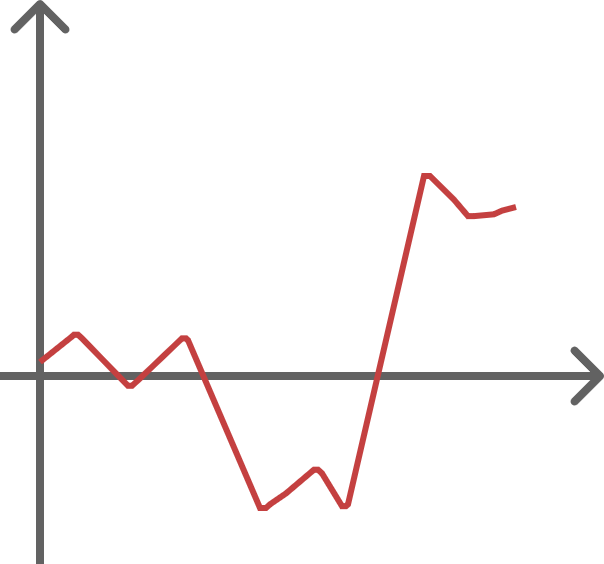
\includegraphics[width=\textwidth]{figures/prelem/timeseries.png}
        \caption{Data Series}
        \label{fig:dataseries}
    \end{subfigure}
    \hfill
    \vspace{1.0cm} 
    \begin{subfigure}[b]{0.35\textwidth}
        \centering
        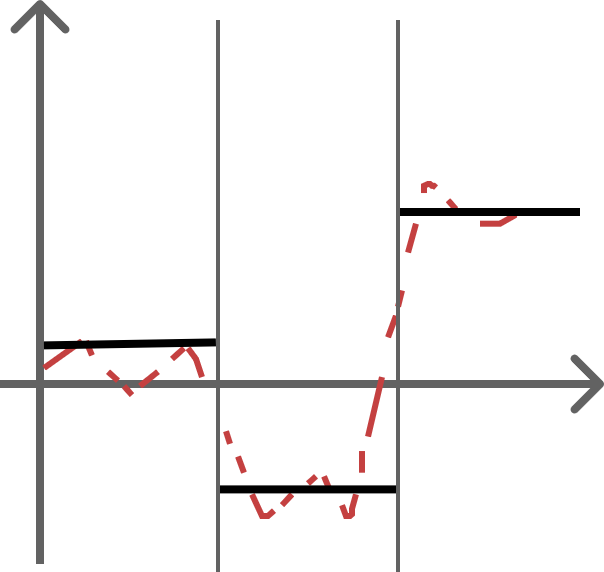
\includegraphics[width=\textwidth]{figures/prelem/PAA.png}
        \caption{PAA Summary}
        \label{fig:PAA}
    \end{subfigure}
    \begin{subfigure}[b]{0.45\textwidth}
        \centering
        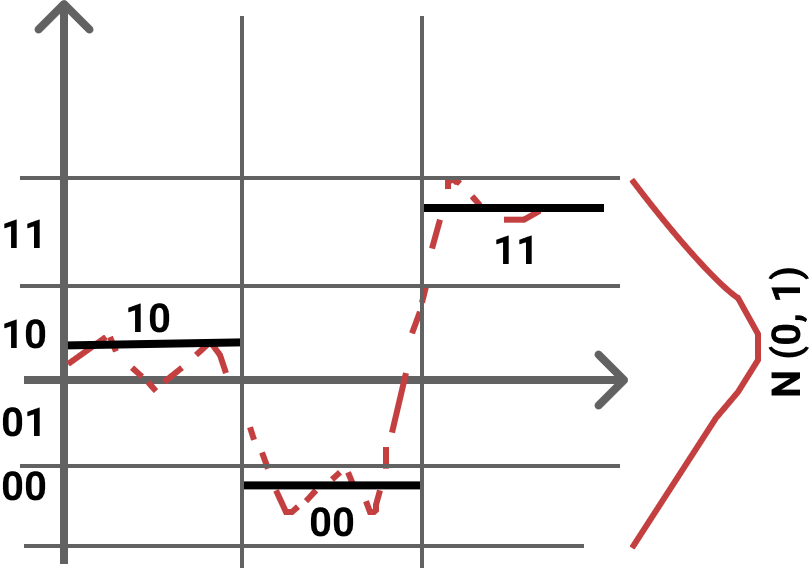
\includegraphics[width=\textwidth]{figures/prelem/isax.png}
        \caption{iSAX Summary}
        \label{fig:iSAXSummary}
    \end{subfigure}
    \vspace{1.0cm} 

    \begin{subfigure}[b]{0.9\textwidth}
        \centering
        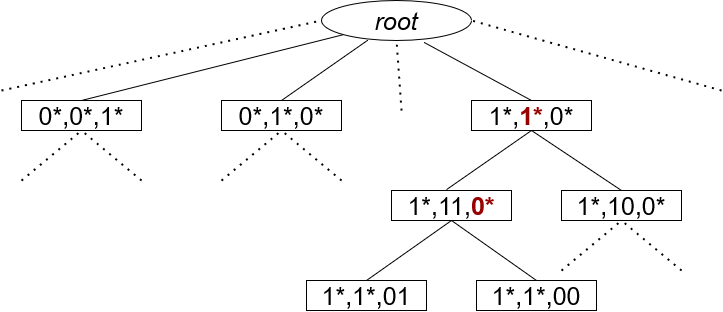
\includegraphics[width=\textwidth]{figures/prelem/isaxTreeCustom.png}
        \caption{iSAX Tree}
        \label{fig:iSAXTree}
    \end{subfigure}

    \caption{From data series to iSAX index}
    \label{fig:from_ds_to_iSAX}
\end{figure}

\noindent{\bf Similarity Search}  
We focus on \textit{exact similarity search} (also known as exact \textit{1-NN}),  
which retrieves the data series from a collection that is most similar to a given 
query series. Similarity is typically measured using \textbf{Euclidean Distance (ED)},
but our techniques are general enough to support other widely used 
\textit{similarity measures}, such as Dynamic Time Warping (DTW)~\cite{rakthanmanon2012searching}.  
% 
The \textbf{Euclidean distance} between two time series  
\( T = \{t_1, ... , t_n\} \) and \( T' = \{t'_1, ... , t'_n\} \)  
is defined as:  
\begin{equation}
ED(T, T') = \sqrt{\sum_{i=1}^{n} (t_i - t'_i)^2}
\label{eq:Euclidean-distance}
\end{equation} 
% 
We refer to the distance between the \textit{iSAX summaries} of two data series  
as the \textbf{lower-bound distance}. If we transform the original subsequences into PAA
representations, $\overline{T}$ and $\overline{T'}$, using Eq.~\ref{eq:paa-transformation}
(according to~\cite{Lin2007SAX}),
we can then obtain a lower bounding approximation of the Euclidean distance
between the original subsequences by:

\begin{equation}
DR(\overline{T}, \overline{T'}) \equiv \sqrt{\frac{n}{w}} \sqrt{\sum_{i=1}^{w} (\overline{t}_{i} - \overline{t'}_{i})^2}
\label{eq:lower-bound-distance}
\end{equation}

% 
The calculation of this distance guarantees the \textbf{pruning property}:  
the lower-bound distance between two data series is always less than or equal to  
their Euclidean distance, which we refer to as the \textbf{real distance}.  
% 
This property enables efficient pruning of candidates during query processing:  
a data series can be \textbf{pruned} if its lower-bound distance to the query series
\( Q \) is greater than the real distance of any other data series in the collection 
from \( Q \).

\noindent
{\bf Leaf-Oriented Trees.}  
In a \textit{leaf-oriented tree}, all data are stored in the leaves, with each leaf
capable of holding up to \( M \) keys.  
% 
During an insertion, if the target leaf \( \ell \) has available space,  
the new key is simply added to \( \ell \).  
However, if \( \ell \) is full, it undergoes a \textbf{split}: it is replaced 
by a subtree consisting of an internal node and two new leaves.  
The keys from \( \ell \) are then redistributed between the new leaves based on
their values.  
% 
If one of the newly created leaves remains empty after redistribution,  
the splitting process is repeated until both leaves contain keys.  

\section{iSAX-Based Indexing}

Concurrent iSAX-based indexes~\cite{peng2018paris,parisplus,peng2020messi,  
PFP21-I,PFP21-II} operate in two main phases:  
the \textit{tree index construction phase} and the \textit{query answering phase},  
each utilizing distinct data structures. 

\noindent\textbf{Tree Index Construction.} During this phase a set of \textit{worker threads}  
processes a collection of input data series (i.e., \textit{raw data}).  
Each series is summarized using an iSAX representation and inserted into a 
\textit{tree index} as a pair of an iSAX summary and a pointer to the corresponding 
data series.  
% 
The process is divided into two main stages:
\begin{itemize} [noitemsep, topsep=3pt, partopsep=0pt, parsep=0pt]
    \item \textbf{Buffers Creation:} iSAX summary pairs are first stored in array-based  
    \textit{summarization buffers}.  
    \item \textbf{Tree Population:} Worker threads traverse these buffers and insert 
    their entries into the tree index.  
\end{itemize}  
Data series with similar iSAX representations are placed in the same buffer and later  
within the same subtree of the index tree.  
This approach ensures \textbf{high parallelism}, \textbf{good locality}, and  
\textbf{low synchronization overhead} during index construction.
\newline\noindent\textbf{Query Answering.}  
Given a query data series \( Q \), the system follows these steps
to find the data series with the smallest distance to \( Q \) :  
\begin{enumerate}[noitemsep, topsep=1pt, partopsep=0pt, parsep=0pt]
    \item The iSAX summary of \( Q \) is computed and used to traverse the index tree,  
    leading to a leaf \( \ell \).  
    \item The \textit{real distance} between \( Q \) and each data series in \( \ell \) is computed.  
    \item The smallest distance found so far is stored in the \textbf{Best-So-Far (BSF)} variable,  
    serving as an initial approximate answer.  
\end{enumerate}  
% 
Then query answering proceeds by exexuting the following two stages
namely the \textit{Prunning Stage} and the \textit{Refinement Stage}:
\newline\noindent\textbf{Pruning Stage.} In this stage, a set of \textit{query answering threads}
traverse the tree. If the \textit{lower bound distance} from a node to $Q$
exceeds the Best So Far (BSF) value, the node is \textit{pruned} and excluded from
further processing. This pruning ensures that no pruned data series can contribute
to the final answer.
\newline\noindent\textbf{Refinement Stage.} During refinement, the non pruned data series 
are the candidate series and are stored in one or more \textit{priority queues}~\cite{parisplus,PFP21-I,PFP21-II}.
Multiple threads process these candidate data series, calculating their exact
distances to Q. The BSF is updated whenever a smaller distance is encountered.
\newline At the end of this phase, the final answer is contained in BSF.  
\textit{Barriers} synchronize threads at the end of each stage, ensuring correctness,  
while \textit{locks} handle concurrent access to shared data structures.  
Figures~\ref{fig:example} and~\ref{fig:example2} summarize the indexing process.  

\begin{figure}[htbp]
    \centering
    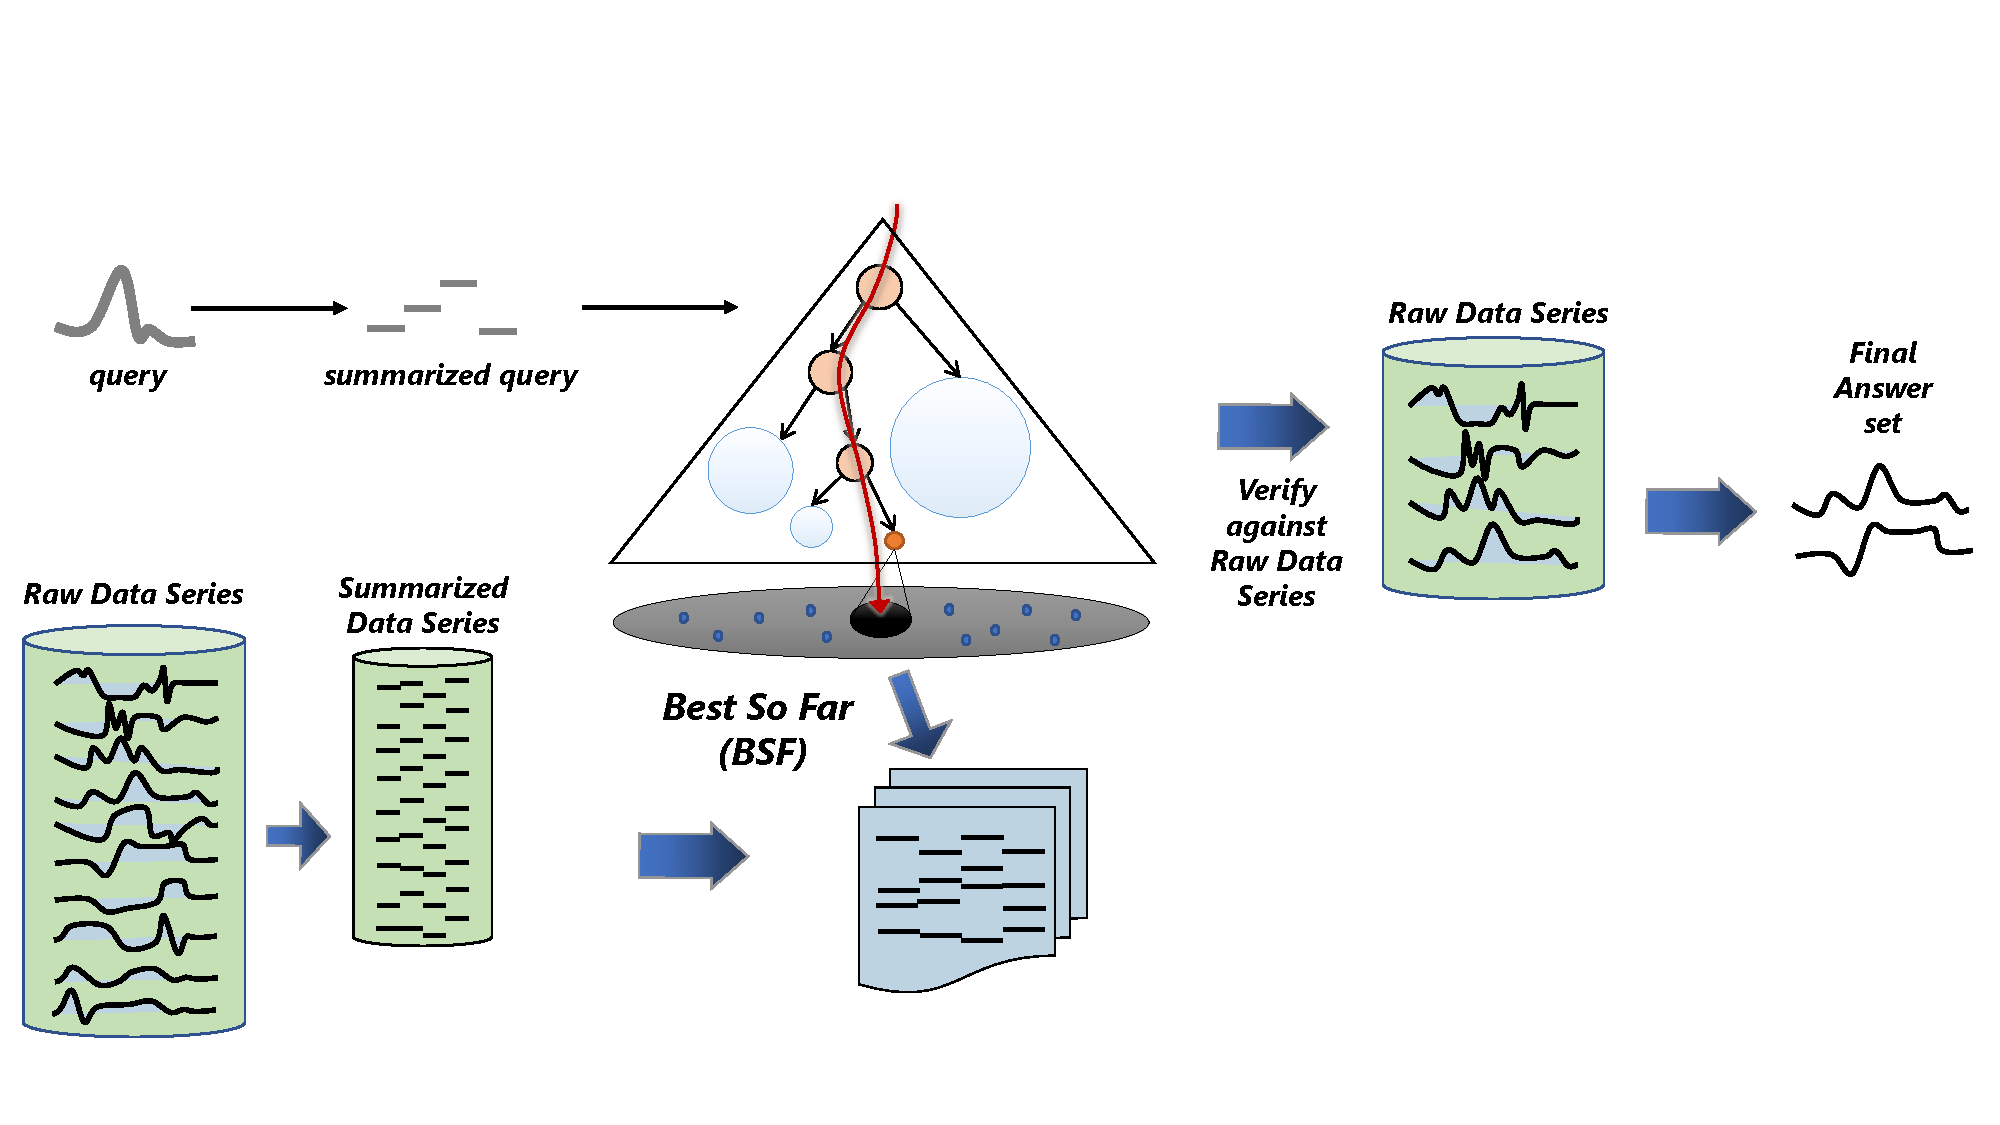
\includegraphics[width=0.85\textwidth]{figures/prelem/iSAX-index.pdf}
    \caption{Similarity search with the use of a data series index.}
    \label{fig:example}
    \vspace{-0.5cm} % Reduces space after the figure
\end{figure}

\begin{figure}[htbp]
    \centering
    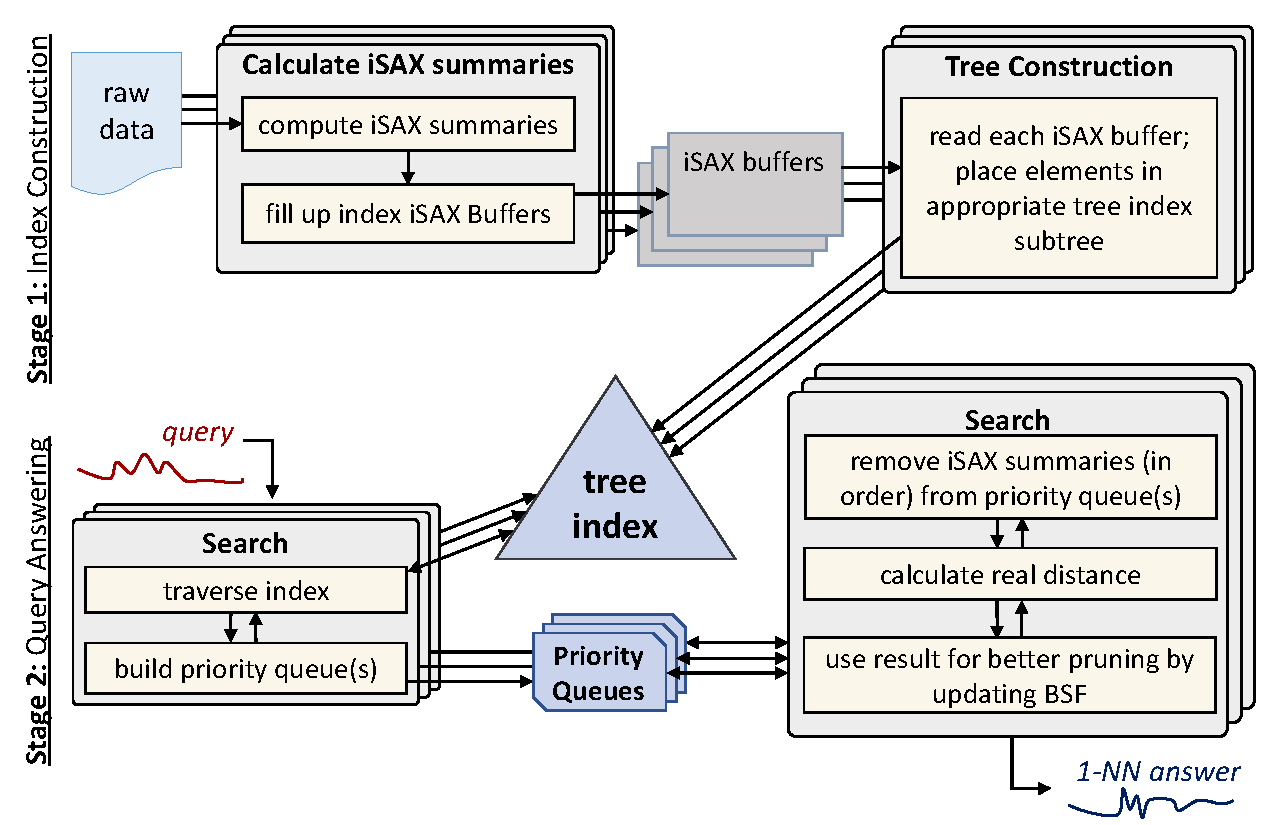
\includegraphics[width=0.8\textwidth]{figures/prelem/flowchart2.pdf}
    \caption{Index building and query answering flowchart for the MESSI data series index.}
    \label{fig:example2}
    \vspace{-0.5cm} % Reduces space after the figure
\end{figure}


\noindent{\bf MESSI as an example.} 
MESSI~\cite{peng2020messi} is a state-of-the-art, in-memory iSAX-based index.
It uses an array, referred to as \textit{RawData}, to store the raw data. During the 
{\em buffers creation stage}, this array is split into a number of fixed-size chunks 
containing consecutive raw data series. A Worker thread repeatedly {\em acquires} and
processes a chunk, storing the calculated iSAX summaries in the appropriate 
summarization buffers. Threads determine which chunks to work on using a \FAI\ object.
Each thread is allocated its own space in each summary buffer to avoid collisions when
adding elements, ensuring thread safety. This process continues until all data series in
\textit{RawData} have been processed.
% 
During the {\em tree population stage}, worker threads again use \FAI\ to {\em acquire}
iSAX buffers to work on. Each subtree of the index tree is a binary leaf-oriented tree
with fat leaves.
% 
In the {\em query answering phase}, a query answering worker repeatedly {\em acquires}
a subtree (using \FAI) and {\em traverses} it by calculating the {\em lower-bound
distance} between the query series \( Q \) and the iSAX summary of each node
encountered. If the lower-bound distance of a leaf is smaller than the Best So Far (BSF)
distance, the leaf is inserted into a {\em priority queue}, with the distance
used as the priority. The algorithm uses a set of {\em priority queues} and threads 
insert elements into these queues in a round-robin fashion.
Since a priority queue may be concurrently accessed by multiple threads, 
MESSI employs a coarse-grain {\em lock} for each queue for synchronization.
% 
During the {\em refinement phase}, each query answering thread \( t \) is assigned a 
priority queue \( \mathit{PQ} \) to process. It repeatedly removes the leaf with the
minimum priority from \( \mathit{PQ} \) and compares its iSAX summary to the BSF.
If the leaf's summary is smaller, the real distances between the data series stored
in the leaf and the query series are computed. Otherwise, the leaf and all remaining
nodes in the queue are pruned. Since multiple threads may process a priority queue
concurrently, it is protected by a coarse-grain lock. Once processing of a priority
queue is complete, thread \( t \) moves on to the next priority queue in a round-robin
manner.
% 
{\em Barriers} are used among threads at the end of each stage and before the start of 
the next to ensure correct synchronization and maintain the integrity of the process.

\section{System And Dynamic Data}
\noindent{\bf System:}
We consider a shared-memory system with \( N \) threads that execute {\em concurrently
and asynchronously} while communicating by accessing shared objects. A shared object
\( O \) can be atomically read or written. Additionally, the operation \FAI(O, v)
atomically reads the current value of \( O \), adds the value \( v \) to it, and
returns the value that was read. The operation \CAS($O, u, v$) reads the value of
\( O \), and if it is equal to \( u \), it changes it to \( v \) and returns
\textit{True}; otherwise, \( O \) remains unchanged and \textit{False} is returned.
% 
Threads may experience delays (e.g., due to page faults, power consumption issues,
or overheating~\cite{inteloverheating}), or they may fail by crashing (e.g., due to
software errors). An algorithm is said to be {\em blocking} if a thread must wait for
actions to be performed by other threads in order to make progress. {\em Lock-freedom}
guarantees that some thread makes progress at each point in time, thus 
the system as a whole continues to make progress independently of the speed of threads
or their failures. Lock-Free algorithms do not utilize locks, MESSI is not lock-free;
it is blocking.


 
\noindent{\bf Dynamic Data:} To simulate dynamicity in data we assume that all data is initially stored in memory, but
only a small subset is used to create the initial index. The rest of the data are organized into batches.
After the initial index is built, new data arrives dynamically in batches, with the batch size
configurable by the user. To simulate real-time data ingestion, we introduce a delay interval
between consecutive batches. This delay, which can be defined by the user,
begins as soon as a batch arrives. By appropriately tuning with the delay we simulate different
dynamicity patterns in data. 
% 
The behavior of the system depends on the interplay between batch size and delay interval.
If the delay is determined to be long enough, index workers (i.e., threads responsible for building the index)
may fully integrate each batch into the index before the next batch arrives, remaining idle for
the rest of the time. Conversely, if the delay is determined to be short or the batch size is large, new batches
may arrive before previous ones have been fully processed.
% 
While index workers are responsible for inserting new data, query workers (i.e., threads
responsible for answering queries) simultaneously access this data to perform
exact similarity search. Ensuring correctness in such a system requires a robust mechanism to
manage concurrent updates and queries. To achieve this, we employ two models inspired by different
domains of computer science: a \textit{timestamp-based model} and a \textit{consistency model based
on linearizability}.  

\subsection{Timestamp-Based Ordering And Linearizability}  

A well-known approach for handling dynamic data is the use of timestamps to enforce ordering 
constraints. This method is widely used in database systems ~\cite{babcock2002} with 
Apache Kafka and Google Spanner~\cite{kafka2021,spanner2013} being example of systems
that employ such mechanisms.  
% 
In our approach, timestamps are implicitly generated using the system's clock. Specifically,
every batch is assigned a timestamp corresponding to the time when the processing of the batch
starts. This timestamp plays a crucial role in  how queries behave. Specifficaly,   

\begin{itemize} [noitemsep, topsep=3pt, partopsep=0pt, parsep=0pt]
    \item Queries must see all data that previous queries have seen.  
    \item If a query has a higher than or equal to timestamp than an ongoing batch, 
    it must wait for that batch to finish processing before continuing.  
\end{itemize}  
% 
By enforcing this ordering, we ensure that queries always operate on a consistent view of the data.
Our approach is inspired by the principles outlined in \textit{Models and Issues in Data Stream
Systems}~\cite{babcock2002}, which guided the design and implementation of timestamps in our dynamic system.  

The second approach we employ is inspired by \textit{linearizability}
\cite{herlihyWingLinearizability}, a key concept in concurrent
and distributed systems. Linearizability provides a strong consistency guarantee by ensuring
that all operations appear to execute atomically in a single, consistent order.  
% 
A system is considered \textbf{linearizable} if:  
 In each execution a, each implemented operation should have the same responce
 as if it has executed serially (or atomically) at some point in its execution
 interval. This point is called linearization point of the opration.

The Timestamp and Linearizability models complement each other by addressing different
aspects of correctness in a dynamic, concurrent system, reflecting the principles of two
distinct domains: the database world and the concurrent computing world.
The timestamp model requires queries to wait for ongoing batches to finish before starting
their processing. This ensures that the data series of any batch arriving before or concurrently 
with a query will be considered when asnwering the query.
This approach respects the temporal sequence of batch arrivals in query processing.
On the other hand, linearizability allows fully concurrent updates and queries with no 
waiting time. While data arrives, the algorithm is responsible for handling it, ensuring that the execution
remains linearizable.
%%%%%%%%%%%%%%%%%%%%%%% Traverse Object %%%%%%%%%%%%%%%%%%%%%%%%%%%%%%%%%%%%%%%%%%%%%%%%%%%%%%%%
\chapter{Traverse Object}
\label{chapter:traverse-object}

\section{Traverse Object}

In this section, we introduce the \textbf{traverse object}, an abstract data type
that enables a modular design for iSAX-based indexes. The processing pipeline of
an iSAX-based index consists of multiple stages, where each stage processes data
produced by the previous one. The first stage handles the original dataset, while
subsequent stages refine and structure the data progressively. This structured
processing inspired the definition of the \textbf{traverse object}, whose
sequential specification is given below.

\subsection{Definition of the Traverse Object}

\begin{definition}
\label{def:traverse}
Let $U$ be a universe of elements. A \textbf{traverse object} $S$ stores elements
of $U$ (which may not be distinct) and supports the following operations:

\begin{itemize}
    \item \textit{Put}($S,e,\mathit{param}$): Adds an element $e \in U$ to $S$.
    The optional parameter $\mathit{param}$ allows implementations to pass
    additional arguments.
    
    \item \textit{Traverse}($S,f,\mathit{fparam},del$): Traverses $S$, applying
    the function $f$ with parameters $\mathit{fparam}$ to each element. If the
    $del$ flag is set, the elements are deleted from $S$ after being processed.
    The parameter $\mathit{fparam}$ serves the same purpose as in \textit{Put}.
\end{itemize}

A traverse object $S$ satisfies the \textbf{traversing property}:  
Each instance of \textit{Traverse} in a sequential execution applies $f$ at
least once to all distinct elements added to $S$ that have not been deleted
in a previous invocation of \textit{Traverse}.
\end{definition}

\subsection{Traverse Objects in iSAX-Based Indexing}

\begin{algorithm}[htbp]
    \footnotesize
    \vspace*{2mm}
    
    \begin{algorithmic}[1]
    
    \Procedure{InitializeSharedObjects}{}
        \State \BC $\gets$ initially contains all raw data series
        \State \TP, \PS, \RS $\gets$ initially empty
        \State $\mathit{BSF} \gets$ some initial value
    \EndProcedure
    
    \vspace*{1mm}
    \State{Code for thread $t_i$, $i \in \{0, \ldots, n-1\}$:}		
    \vspace*{1mm}

    \Procedure{\QueryAnswering(QuerySeriesSet $\mathit{SQ}$) \textbf{returns} int}{}
        \State \BC.\Traverse(\&BufferCreation(), $\mathit{BCParam}$, \False)
        \State \TP.\Traverse(\&TreePopulation(), $\mathit{TPParam}$, \False)
        \State \PS.\Traverse(\&Prunning(), $\mathit{PSParam}$, \False)
        \State \RS.\Traverse(\&Refinement(), $\mathit{RSParam}$, \True)
        \State \Return $\mathit{BSF}$
    \EndProcedure
    
    \vspace*{1mm}
    \Procedure{\BufferCreation(DataSeries $\mathit{ds}$)}{}
        \State iSAXSummary $\mathit{iSAX} \gets$ Calculate the iSAX summary for $\mathit{ds}$
        \State Index $\mathit{bind} \gets$ index to appropriate buffer based on $\mathit{iSAX}$
        \State \TP.\Put($\langle \mathit{iSAX}$, index of $\mathit{ds}$ $\rangle$, $\mathit{bind}$)
    \EndProcedure
    
    \vspace*{1mm}
    \Procedure{\TreePopulation(Summary $\mathit{iSAX}$, Index $\mathit{ind}$,
         Index $\mathit{bind}$, Boolean $\mathit{flag}$)}{}
        \State \PS.\Put($\langle \mathit{iSAX}$, $\mathit{ind} \rangle$, $\mathit{bind}$, $\mathit{flag}$)
    \EndProcedure
    
    \vspace*{1mm}
    \Procedure{\Prunning(DataSeries $Q$, DataSeriesSet $\mathit{E}$, Boolean
        $\mathit{flag}$) \textbf{returns} boolean}{}
            \State iSAXSummary $\mathit{iSAX} \gets$ Calculate the iSAX summary for $\mathit{E}$
            \State int $\mathit{lbDist} \gets$ lower bound distance between $\mathit{iSAX}$ and $Q$
            \If{$\mathit{lbDist} < \mathit{BSF}$}
                \State \RS.\Put($\langle \mathit{E, iSAX} \rangle$, $\mathit{flag}$)
                \Return \True
            \EndIf
            \Return \False
    \EndProcedure
    
    \vspace*{1mm}
    \Procedure{\Refinement(DataSeries $Q$, DataSeriesSet $E$, Summary $\mathit{iSAX}$,
     Function *\UpdateBSF) \textbf{returns} Boolean}{}
        \State int $\mathit{lbDist}$, $\mathit{rDist}$
        \State $\mathit{lbDist} \gets$ lower bound distance between $\mathit{iSAX}$ and $Q$
        \If{$\mathit{lbDist} < \mathit{BSF}$}
            \ForAll{pair $\langle \mathit{iSAX_{ds}, ind_{ds}} \rangle$ in $E$}
                \State $\mathit{lbDist} \gets$ lower bound distance between $\mathit{iSAX_{ds}}$ and $Q$
                \If{$\mathit{lbDist} < \mathit{BSF}$}
                    \State $\mathit{rDist} \gets$ real distance between $\mathit{ds}$ and $Q$
                    \If{$\mathit{rDist} < \mathit{BSF}$}
                        \State *\UpdateBSF($\mathit{BSF},\mathit{rDist}$) \Comment{user-provided routine}
                    \EndIf
                \EndIf
            \EndFor
            \Return \True
        \Else
            \Return \False
        \EndIf
    \EndProcedure
    
    \end{algorithmic}
    
    \caption{Implementation of an iSAX-based index using the traverse objects \BC, \TP, \PS, \RS.}
    \label{alg:iSAXTraverse}
    \end{algorithm}
    
    


To implement the different stages of an iSAX-based index, we use four instances of a traverse object 
to store and manipulate different types of data:

\begin{itemize}
    \item \textbf{Buffer Creation ($BC$)}: Stores the raw data series.
    \item \textbf{Tree Population ($TP$)}: Stores pairs of iSAX summaries and
     pointers to data series.
    \item \textbf{Pruning ($PS$)}: Organizes these pairs into sets corresponding
     to the leaf nodes of the tree.
    \item \textbf{Refinement ($RS$)}: Maintains priority queues of candidate
     series for query answering.
\end{itemize}

Each of these objects plays a crucial role in the indexing and query answering
process. The \textbf{buffer creation} phase utilizes an array, \RawData, to 
store the raw data series. Thus, elements of $BC$ are stored in \RawData. 
The \textbf{tree population} phase employs a set of \textbf{summarization buffers},
where iSAX summaries and pointers are initially stored. The traverse object $TP$
holds these pairs. The \textbf{pruning} stage organizes these pairs within a
leaf-oriented tree, where $PS$ manages sets of pairs corresponding to each tree leaf. 
Finally, the \textbf{refinement} phase employs priority queues to manage tree
leaves containing candidate series for further evaluation.

\subsection{Query Answering as a Sequence of Traversals}

Query answering in an iSAX-based index follows a structured sequence of four
\textit{Traverse} operations, applied in order to the different traverse objects.  
Algorithm~\ref{alg:iSAXTraverse} presents the pseudocode for implementing an iSAX-based index
using traverse objects.

Since the four stages do not overlap, their execution is typically synchronized
using barriers. In Algorithm~\ref{alg:iSAXTraverse}, these barriers (as well as any 
multithreading aspects) are embedded within the implementations of \textit{Put}
and \textit{Traverse}. This ensures that an iSAX-based index satisfies the
following key property:

\begin{definition}[\textbf{Non-Overlapping Property}]
\label{def:non-overlapping}
In every concurrent execution of the index, for every traverse object $S$, an
instance of \textit{Traverse} on $S$ is performed only after all \textit{Put}
operations that add distinct elements to $S$ have completed.
\end{definition}

\subsection{Ensuring Correctness Through Traversing and Non-Overlapping Properties}

Assuming that the \textbf{non-overlapping property} holds for $BC$, $TP$, $PS$,
and $RS$, and that \RawData initially contains all data series in the collection,
the \textbf{traversing property} guarantees that:

\begin{enumerate}
    \item The \BufferCreation function is invoked at least once for each data
     series in \RawData.
    \item The corresponding iSAX summary is computed, ensuring that at least one
     appropriate pair is inserted into $TP$.
    \item By the \textbf{non-overlapping property}, the \TreePopulation function
     processes all these pairs, inserting them into $PS$ (the index tree).
    \item The \Prunning function is applied to all elements in $PS$, and leaves
     that cannot be pruned are inserted into $RS$.
    \item The \Refinement function is applied to every traversed element of $RS$.
     Since \textit{Traverse} on $RS$ is invoked with $del = \mathit{True}$,
    priority queues can be used to implement $RS$, and \DeleteMin can be employed
    to remove elements as they are processed.
\end{enumerate}

Thus, the system ensures that only relevant candidates are further processed,
refining the query results by computing exact distances and updating the
\textbf{best-so-far} ($BSF$) value when necessary.

Implementations of \textit{Put} and \textit{Traverse} for $BC$, $TP$, $PS$, and
$RS$ in FreSh are provided in chapter~\ref{chapter:FreSh}.

\bl{
\section{Adapting the Traverse Object for Dynamic Data Processing}  

To support dynamic data processing in an iSAX-based index, the
\textit{traverse object} requires adaptation. In a dynamic setting,
threads execute concurrently and independently across the two distinct phases
of the index: \textit{index creation} and \textit{query answering}.
Consequently, the \BC\ and \TP\ traverse objects are assigned to the
\textit{index workers} (threads responsible for constructing the index), while
the \PS\ and \RS\ traverse objects are assigned to the \textit{query workers}
(threads responsible for answering queries).  

\subsubsection{Impact of Concurrency on Traverse Objects}  

The concurrent execution of these phases alters the procedure for answering
queries using traverse objects (see Algorithm~\ref{alg:DynamiciTraverseObject}).
Unlike the static setting, where the procedure involves four sequential
invocations of \Traverse\ (one for each traverse object), in the dynamic
setting, the sequence is reduced to only the last two traverse objects,
\PS\ and \RS.  

This change directly affects the \textit{non-overlapping property}
(Definition~\ref{def:non-overlapping}), which now applies only to traverse
objects within the same phase:  
\begin{itemize}  
    \item \textbf{Index workers:} \BC\ and \TP  
    \item \textbf{Query workers:} \PS\ and \RS  
\end{itemize}  

Since \Traverse\ and \Put\ operations can occur concurrently across phases,
situations arise where an index worker inserts new elements into the iSAX tree
while query workers are simultaneously pruning or refining their results.
This requires additional mechanisms to maintain correctness.  

\subsubsection{Handling Multiple Batches}  

In a dynamic environment where data arrives in batches, certain data structures
implementing traverse objects—specifically, \BC\ and \PS—must be
\textit{re-initialized} before processing a new batch. This re-initialization
is necessary because:  
\begin{itemize}  
    \item Each batch reuses the same buffers, meaning helpers must distinguish
    between \textbf{current} and \textbf{obsolete} data.  
    \item Helpers need to \textbf{skip outdated data} that no longer belongs to
    the active batch.  
    \item This differentiation is particularly important during the traversal of
    \TP\ and \PS\ objects.  
\end{itemize}  

\subsubsection{Ensuring Correctness with Sequence Numbers}  

To address these challenges, our approach introduces \textit{sequence numbers}
as a mechanism to track the state of the algorithm.  

\begin{definition}  
A \textbf{sequence number} is a monotonically increasing integer used to track  
the order of operations and ensure consistency in multi-threaded or
distributed environments.  
\end{definition}  

Each \textit{summarization buffer} is associated with a sequence number.
During \textbf{re-initialization}, an index worker performs the following steps:  
\begin{enumerate}  
    \item Resets the buffer size to zero.  
    \item Increments the buffer's sequence number by one.  
\end{enumerate}  

This mechanism prevents a thread from processing outdated data. If a worker reads
a nonzero buffer size, it indicates the presence of data. However, before proceeding,
the worker also checks the \textbf{sequence number}:  
\begin{itemize}  
    \item If the sequence number \textbf{matches} the current batch ID,
     the data is valid and can be processed.  
    \item If the sequence number is \textbf{smaller} than the current batch ID,
     the data is obsolete and must be ignored.  
\end{itemize}  

This ensures that no worker mistakenly processes data from a previous batch
(see Algorithm~\ref{alg:BufferReuse}).  


\begin{algorithm}[htbp]
    \footnotesize
    \vspace*{2mm}
    
    \begin{algorithmic}[1]
    
    \Procedure{InitializeSharedObjects}{}
        \State \BC $\gets$ initially contains all raw data series
        \State \TP, \PS, \RS $\gets$ initially empty
        \State $\mathit{BSF} \gets$ some initial value
        \State $\mathit{NextUpdateAvailable} \gets 0$
        \State $\mathit{GlobalSeq} \gets 0$
    \EndProcedure
    
    \vspace*{1mm}
    \State{Code for thread $t_i$, $i \in \{0, \ldots, k-1\}$:}    
    \vspace*{1mm}
    
    \Procedure{IndexCreation(int $\mathit{TotalUpdates}$) \textbf{returns} int}{}
        \State int $\mathit{currentBatch} \gets 1$
        \While{$\mathit{currentBatch} < \mathit{TotalBatches}$}
            \If{$\mathit{model} == \mathit{SystemTS}$ }
                \State batchTS $\gets$ getTS()
            \EndIf
            \State \BC.\Traverse(\&BufferCreation(), $\mathit{BCParam}$, \False)
            \State \TP.\Traverse(\&TreePopulation(), $\mathit{TPParam}$, \False)
            \ForAll{summarization buffers that have data}
                \State ReuseBuffers($\mathit{summBuffer}, \mathit{currentBatch}$)
            \EndFor
            \If{$\mathit{DELAY} >= \mathit{BatchProcessingTime}$}
                \State sleep($\mathit{DELAY}-\mathit{BatchProcessingTime}$)
            \EndIf
            \State $\mathit{currentBatch} \gets \mathit{currentBatch} + 1$
        \EndWhile
    \EndProcedure
    
    \vspace*{1mm}
    \State{Code for thread $t_i$, $i \in \{k, \ldots, n-1\}$:}    
    \vspace*{1mm}
    
    \Procedure{QueryAnswering(QuerySeriesSet $\mathit{SQ}$) \textbf{returns} int}{}
        \State int $\mathit{localTS} \gets 0$
        \While{$\mathit{!SQ.Empty}$}
            \If{$\mathit{model} == \mathit{LogicalTS}$}
                \If{$\mathit{localSeq} == \mathit{GlobalSeq}$}
                    \State \CAS(\&GlobalSeq, localSeq, localSeq + 1)
                \EndIf
            \ElsIf{$\mathit{model} == \mathit{SystemTS}$}
                \State queryTS $\gets$ getTS()
                \While {$\mathit{queryTS} >= \mathit{batchTS}$}
                    \State backoff()
                \EndWhile
            \EndIf
            \State \PS.\Traverse(\&Pruning(), $\mathit{PSParam}$, \False)
            \State \TP.\Traverse(\&Refinement(), $\mathit{RSParam}$, \False)
            \ForAll{summarization buffers that have data}
                \State ReuseBuffers($\mathit{summBuffer}, \mathit{currentBatch}$)
            \EndFor
            
            \If{$\mathit{model} == \mathit{LogicalTS}$}
                \State $\mathit{localSeq} = \mathit{localSeq} + 1$            
            \EndIf
        \EndWhile
        \State \Return $\mathit{BSF}$
    \EndProcedure
    
    \vspace*{1mm}
    \Procedure{ReuseSumBuffers(SumBuff * $\mathit{currBuff}$, int $\mathit{currentBatch}$)}{} \label{alg:BufferReuse}

        \State $\mathit{currBuff->size[workerID]} \gets 0$
        \If{$\mathit{currBuff->seq[workerID]} < \mathit{currentBatch}$}
            \State $\mathit{currBuff->seq[workerID]} \gets \mathit{currentBatch}$
        \EndIf
        \State $\mathit{currBuff->seq[workerID]++}$
    \EndProcedure
    
    \end{algorithmic}
    
    \caption{Implementation of a dynamic iSAX-based index using the traverse objects \BC, \TP.}
    \label{alg:DynamiciTraverseObject}
    \end{algorithm}
}
%%%%%%%%%%%%%%%%%%%%%%% Locality Awareness %%%%%%%%%%%%%%%%%%%%%%%%%%%%%%%%%%%%%%%%%%%%%%%%%%%%%
\chapter{Locality-Awareness}
\label{chapter:Locality-aware}

\begin{figure*}[tb]
	\centering
	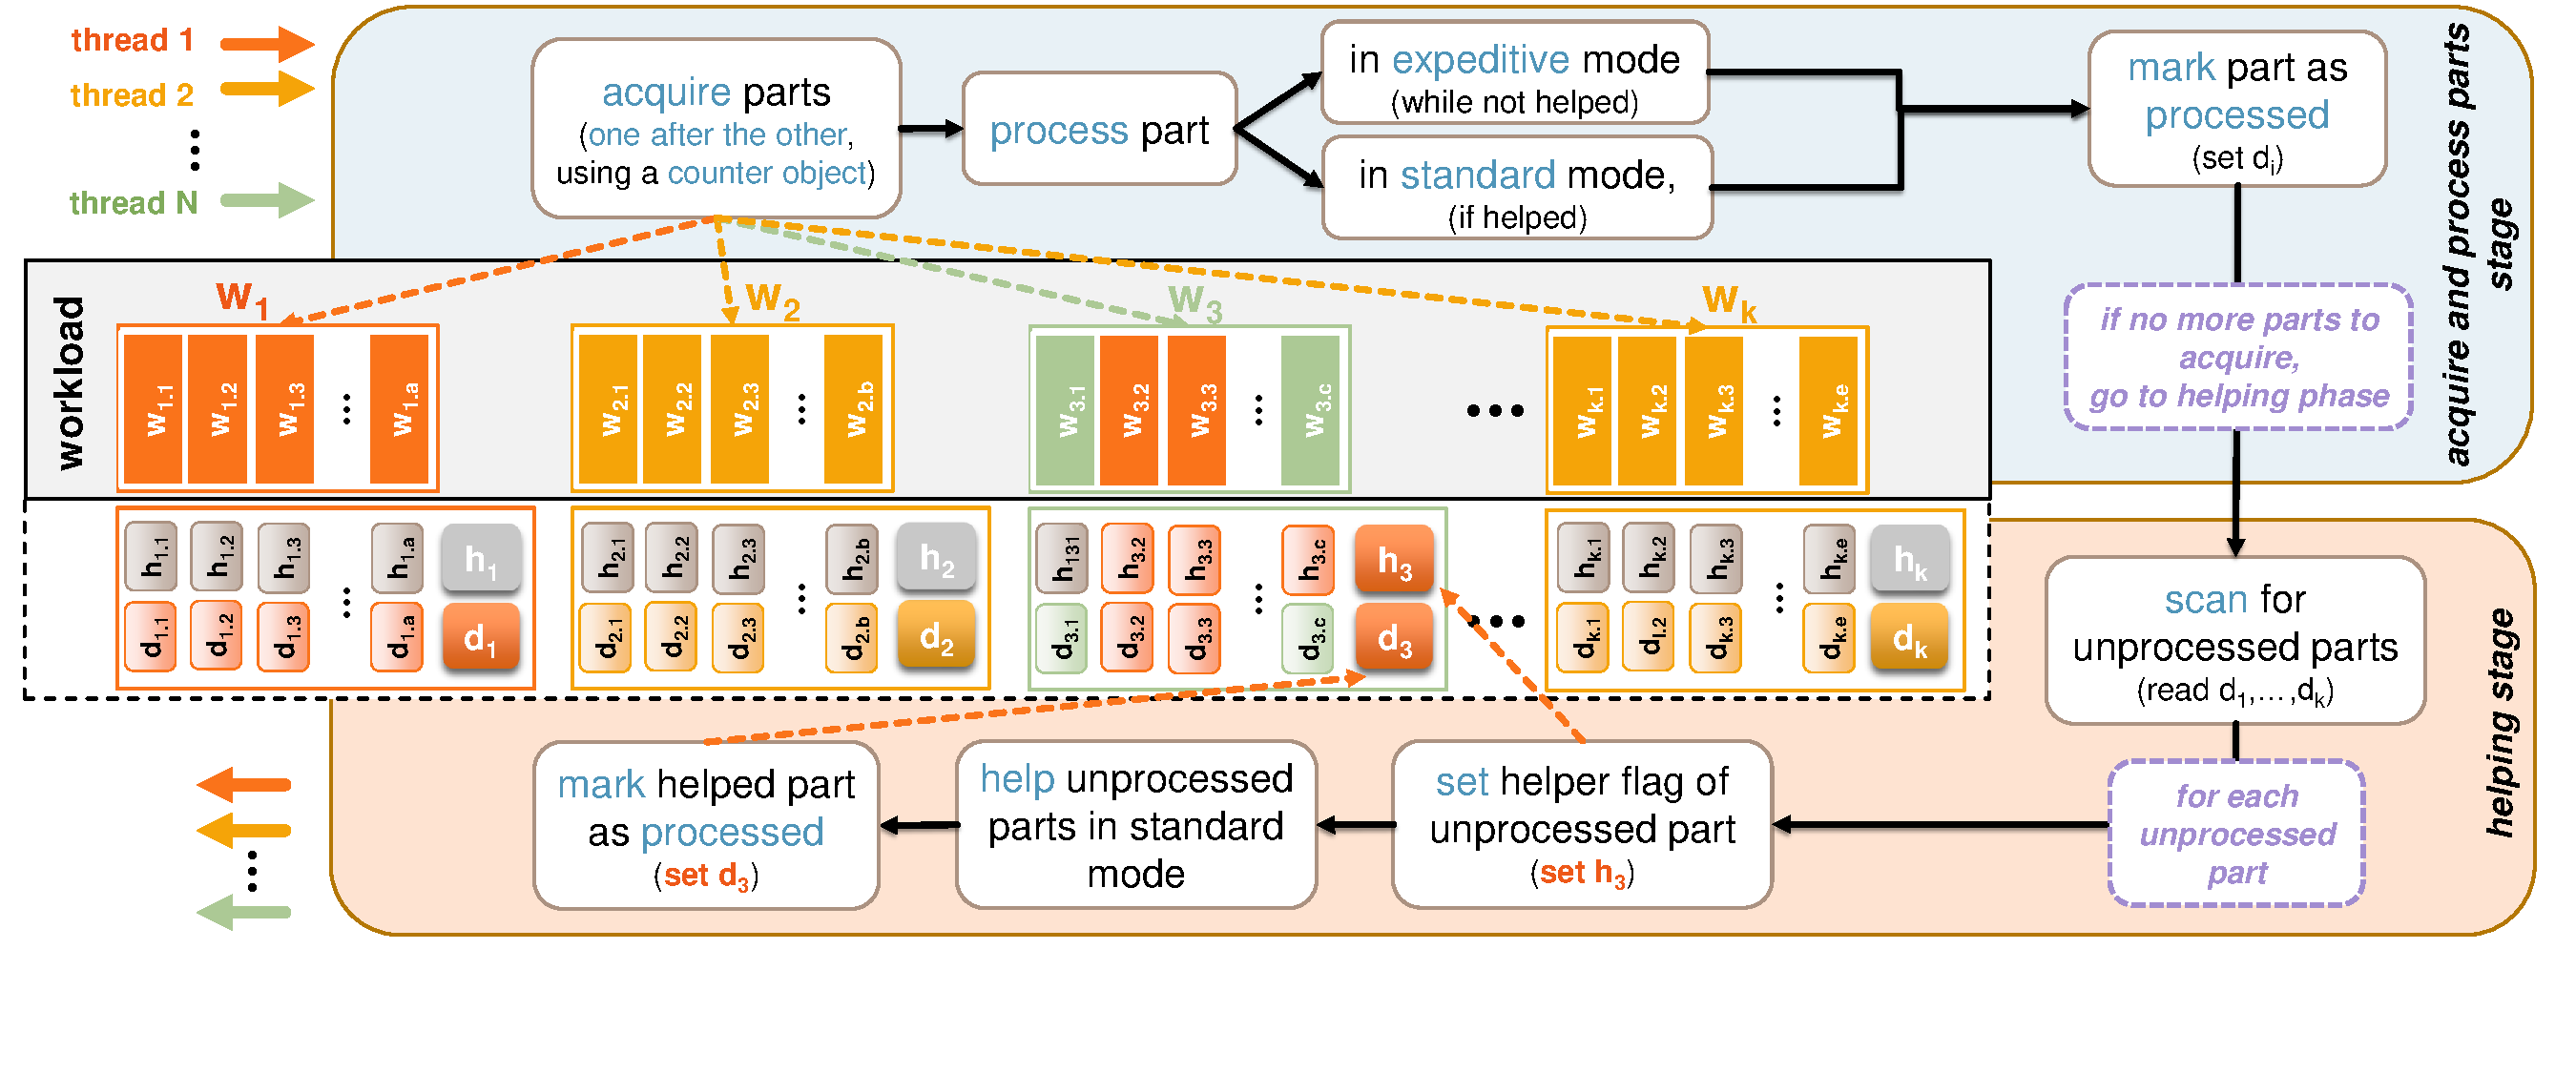
\includegraphics[width=0.9\textwidth]{figures/locality-aware/Refresh_ekosmas_2-Themis.pdf}	
	\vspace*{-0.8cm}
	\caption{Refresh flowchart.}
	\vspace*{-0.2cm}
	\label{fig:refresh:flowchart}
\end{figure*}


{\em Locality-awareness}  aims at capturing several design principles (Definition~\ref{def:principles})
for data series indexes which are crucial for achieving good performance.
A locality aware implementation respects these principles. 
% 
\begin{definition}
\label{def:principles}
Principles for {\em locality-aware} processing:
\begin{enumerate}
\item
{\bf Data Locality.} Separate the data into {\em disjoint sets} and have a distinct thread
processing the data of each set. This results in reduced communication 
cost (cache misses and branch misprediction) among the threads.
\item
{\bf High Parallelism \& Low Synchronization Cost.} 
Threads should work in parallel and independently from each other as much as possible. 
Whenever synchronization cannot be avoided, design the appropriate 
mechanisms to minimize its cost.
\item
{\bf Load Balancing.} Share the workload equally to the different threads, thus
avoiding load imbalances between threads and having all threads busy at each
point in time. 

\end{enumerate}
\end{definition}
% 
Enuring locality awareness results in good performance and is thus 
a desirable property for big data processing. In existing iSAX-based indexes, 
a thread operates on chunks of \textit{RawData} and processes disjoint sets of summarization
buffers and subtrees of the index tree. Also, an iSAX-based index employs 
several priority queues to store leaf nodes containing candidate series.
Thus, iSAX-based indexes are {\em locality-aware}.
% 
To describe \textit{ReFreSh} in more detail, consider a {\em blocking} locality-aware
implementation $\mathcal{A}$, which splits its workload into disjoint parts and assigns them to 
threads for processing. 
% 
The main idea behind it is to require from each thread that completes processing
its own workload,(instead of blocking, waiting for other threads to also finish), 
to scan for unprocessed workloads (e.g. in an iSAX-based index, unprocessed parts of $RawData$
or unprocessed summarization buffers), and help completing their processing. 

\textit{ReFreSh} (Algorithm~\ref{alg:refresh}) transforms $\mathcal{A}$ into a {\em lock-free} 
locality-aware implementation $\mathcal{B}$ that achieves high parallelism. 
% 
Let $W$ be the workload that $\mathcal{A}$ processes 
and let $w_1, \ldots, w_k$ be the parts it is separated to ensure locality awareness.
\textit{ReFreSh} applies for each data structure $D$ of $\mathcal{A}$, 
the following steps (depicted in Figure~\ref{fig:refresh:flowchart}):


%%%%%%%%%%%%%%%%%%%%%%%%%%%%%%% REFRESH ALGORITHM %%%%%%%%%%%%%%%%%%%%%%%%%%%%%%%%%%%%%% 

\begin{algorithm}[htbp]
    \footnotesize
    \vspace*{2mm}
    
    \begin{algorithmic}[1]
    
    \Procedure{InitializeSharedVariables}{}
        \State Workload part $\mathit{W} \gets [w_1, w_2, \ldots, w_k]$ \label{alg:refresh:w}
        \State Boolean array $\mathit{F} \gets [d_1, d_2, \ldots, d_k]$, initially $d_i = \False$ \label{alg:refresh:d}
        \State Boolean array $\mathit{H} \gets [h_1, h_2, \ldots, h_k]$, initially $h_i = \False$ \label{alg:refresh:h}
    \EndProcedure
    
    \vspace*{1mm}
    \State{Code for each thread:}    
    \vspace*{1mm}
    
    \Procedure{Refresh}{}
        \While{$\mathit{W}$ has available parts}  \label{alg:refresh:process:start}
            \State $\mathit{w_i} \gets$ Acquire an available part of $\mathit{W}$
            \State Mark $\mathit{w_i}$ as acquired
            \If{$h_i == \False$}  \label{alg:refresh:process:if}
                \State Process $\mathit{w_i}$ in expeditive mode, while checking that $h_i$ remains $\False$ \label{alg:refresh:process:expeditive}
                \State If $h_i == \True$, switch to standard mode
            \Else
                \State Process $\mathit{w_i}$ in standard mode \label{alg:refresh:process:standard}
            \EndIf
            \State $d_i \gets \True$ \label{alg:refresh:d:true}
        \EndWhile
        
        \vspace*{1mm}
        \ForAll{$d_i \in D$ where $d_i == \False$}  \label{alg:refresh:scan:ForAll} 
            \State Backoff()  \Comment{Avoid helping, if possible} \label{alg:refresh:help:backoff}
            \If{$d_i == \False$}  \label{alg:refresh:help:if}
                \State $h_i \gets \True$ \label{alg:refresh:h:true}
                \State Process $\mathit{w_i}$ in standard mode, checking periodically if $d_i$ remains $\False$ \label{alg:refresh:help:process}
                \State If $d_i == \True$, stop processing $\mathit{w_i}$
                \State $d_i \gets \True$ \label{alg:refresh:help:d:true}
            \EndIf
        \EndFor
    \EndProcedure
    
    \end{algorithmic}
    
    \caption{\textit{ReFreSh} - A general approach for transforming a blocking data structure $\mathit{D}$ into a lock-free one.}
    \label{alg:refresh}
\end{algorithm}

\newpage

\begin{enumerate}
    \item It attaches a {\em flag} $d_i$, $1 \leq i \leq k$, (initially \False)  
    with each $w_i$ to identify whether $w_i$'s processing is done.  
    As soon as a thread finishes processing $w_i$, it sets $d_i$ to \True\ (line~\ref{alg:refresh:d:true}).  

    \item Threads in $\mathcal{B}$ execute the same algorithm as in $\mathcal{A}$ to acquire parts of $W$ to process,  
    until all parts have been acquired (lines~\ref{alg:refresh:process:start}-\ref{alg:refresh:d:true}).  
    The thread that acquires a workload is its {\em owner}.  

    \item To achieve lock-freedom, every thread $t$, then, {\em scans} all the flags ($d_i$, $1 \leq i \leq k$)  
    to find those parts that are still unfinished (line~\ref{alg:refresh:scan:ForAll}).  

    \item Thread $t$ {\em helps} by processing, one after the other, each part found unfinished during scan.  
    For each part $w_i$, $1 \leq i \leq k$, that $t$ helps, it periodically checks $d_i$  
    to see whether other threads completed the processing of $w_i$. If this is so,  
    $t$ stops helping $w_i$ (line~\ref{alg:refresh:help:process}).  
    A thread that completes the processing of $w_i$ changes $d_i$ to \True\ (line~\ref{alg:refresh:help:d:true}).  

    \item Due to helping, every data structure $D$, employed in $\mathcal{A}$, may be  
    concurrently accessed by many threads. Thus, $\mathcal{B}$ should provide an efficient  
    lock-free implementation for all data structures of $\mathcal{A}$.  
\end{enumerate}


In locality-aware implementations, (e.g., in iSAX-based indexes), threads are expected to work
on their own parts of the data most of the time ({\em contention-free phase}), and they
may help other threads only for a small period of time at the end of their execution
({\em concurrent phase}).
In the contention-free phase, \textit{ReFreSh} avoids synchronization overheads incurred to
ensure lock-freedom. 
Specifically, it employs two implementations for each data strucutre $D$ of  $\mathcal{A}$,
one with low synchronization cost that does not support helping ({\em expeditive mode}),
and another that supports helping and has higher synchronization overhead ({\em standard mode}).  
To enable threads operate on the appropriate mode,  a {\em helping-indicator flag} $h_i$ 
(initially \False) , $1 \leq i \leq k$, is attached with each $w_i$. , which indicates whether 
$w_i$'s processing should be performed on expeditive or standard mode.
% 
A thread $t$ starts by processing its assigned workload 
on expeditive mode (lines~\ref{alg:refresh:h} and \ref{alg:refresh:process:if}-\ref{alg:refresh:process:expeditive}).
Before $t$ starts helping some part $w_i$, it sets $h_i$ to \True\ (line~\ref{alg:refresh:h:true}),
to alert $w_i$'s owner thread to start running on standard mode (line~\ref{alg:refresh:process:expeditive}).

To avoid helping whenever it is not absolutely necessary, i.e. when no thread has
failed (or is extremely slow), \textit{RefreSh} provides an optional {\em backoff scheme} that is used
by every thread $t$ (line~\ref{alg:refresh:help:backoff}) 
before it attempts to help other threads (line~\ref{alg:refresh:help:if}-\ref{alg:refresh:help:process}).
A small delay before switching to standard mode, often positively affects performance.
The delay is usually an estimate of the actual time a thread requires to finish its
current workload, calculated at run time.
% 
To minimize the work performed by a helper, \textit{ReFreSh} could
be applied  {\em recursively} by splitting each part $w_i$ to subparts. 
This way, a helper helps only the remaining unfinished subparts of $w_i$.
and not the whole $w_i$. Thus, the redundant work is further decreased. 
To achieve this, the subparts of $w_i$ should have their own flag and helping-indicator variables.

Lock-freedom is ensured due to the {\em helping code} (lines~\ref{alg:refresh:scan:ForAll}-
\ref{alg:refresh:help:d:true}), In \textit{ReFreSh}, only after a thread
$t$ processes a workload $w_i$, it sets $h_i$ to \True\, and $t$ performs 
the helping code after finishing with their assigned workloads. Thus, when $t$ completes
its helping code the processing of all parts of the workload has been completed. 
This means that $t$ may continue directly to the execution of the next stage, without
waiting for the other threads to complete the execution of the current stage. 
Therefore, this scheme renders the use of barriers useless, as needed to achieve lock-freedom. 

Summarizing, \textit{ReFreSh} is a general scheme for processing a locality-aware workload in a
lock-free way, without sacrificing locality-awareness. 

\bl{
\subsection{\textbf{ReFreSh with Dynamic Batches}}  

\textit{ReFreSh} is designed to be applied once per workload. Threads begin execution in 
\textit{expeditive mode} and switch to \textit{standard mode} when a helper arrives. However,
in an iSAX-based index, \textit{ReFreSh} is applied to multiple phases, including the
RawData array, summarization buffers, the iSAX tree, and the sorted arrays.  
When data arrives dynamically in batches, \textit{ReFreSh} must be applied separately for each phase
and its corresponding data structures. For data structures accessed only once per batch (e.g.,
the RawData array), this does not introduce issues. However, for data structures accessed
multiple times (e.g., summarization buffers and the iSAX tree), a challenge arises.  
% 
The core issue lies in how \textit{ReFreSh} determines when to switch execution modes.
Its behavior relies on boolean flags that initially have a value of \texttt{False} and transition
to \texttt{True} during processing. After processing the first batch, subsequent batches will
encounter these flags already set to \texttt{True}, causing \textit{ReFreSh} to always run
in \textit{standard mode}. This is suboptimal because \textit{standard mode} enables helping,
which is unnecessary unless a helper has actually arrived. To maintain performance,
\textit{ReFreSh} must be modified to support batch processing effectively.  

\subsubsection{\textbf{Modifications to Support Batches}}  

To ensure \textit{ReFreSh} works correctly with dynamic batches, we introduce the following
modifications:  

\begin{enumerate}  
    \item \textbf{Replacing Boolean Flags with Counters:}  
    Instead of using boolean flags, we replace them with counters. Each part $w_i$, where $1 \leq i
    \leq k$, is assigned a counter $d_i$ (initially set to 0). This counter tracks whether $w_i$ has
    completed processing for a specific batch. Once a thread finishes processing $w_i$, it
    sets $d_i$ to $\mathit{currentBatch} + 1$, which corresponds to the ID of the next
    batch (see Algorithm~\ref{alg:DRefresh}).  

    \item \textbf{Batch-Aware Execution of \textit{ReFreSh}:}  
    \textit{ReFreSh} is executed once per batch. Each time it runs, it requires the ID of the
    batch it is processing. The counter values are interpreted accordingly:  
    \begin{itemize}  
        \item A part $w_i$ is considered processed for a batch with ID $X$ when $d_i = X + 1$.  
        \item A helper has arrived at part $h_i$ for an update batch with ID $X$ when $h_i = X + 1$.  
    \end{itemize}  
\end{enumerate}  

By implementing these modifications, \textit{ReFreSh} maintains its efficiency across
multiple dynamic batches while ensuring that execution mode transitions occur only when necessary.


%%%%%%%%%%%%%%%%%%%%%%%%%%%%%%% Dynamic Refresh %%%%%%%%%%%%%%%%%%%%%%%%%%%%%%%%%%%%%%%%

\begin{algorithm}[htbp]
    \footnotesize
    \vspace*{2mm}
    
    \begin{algorithmic}[1]
    
    \State \textbf{Shared variables:}
    \State Workload part $\mathit{W} := \mathit{[w_1, w_2, \ldots, w_k]}$ \label{alg:DRefresh:w}
    \State \textbf{int} $\mathit{F} := \mathit{[d_1, d_2, \ldots, d_k]}$, initially $\mathit{d_i} = 0, \forall i \in [1, k]$ \label{alg:DRefresh:d}
    \State \textbf{int} $\mathit{H} := \mathit{[h_1, h_2, \ldots, h_k]}$, initially $\mathit{h_i} = 0, \forall i \in [1, k]$ \label{alg:DRefresh:h}
    
    \vspace*{1mm}
    \State \textbf{Code for each thread:}
    
    \Procedure{DRefresh}{int $\mathit{currentBatch}$}
        \While{$\mathit{W}$ has available parts} \label{alg:DRefresh:process:start}
            \State $\mathit{w_i} \gets$ acquire an available part of $\mathit{W}$
            \State Mark $\mathit{w_i}$ as acquired
            \If{$(\mathit{h_i} == \mathit{currentBatch})$ \textbf{or} $(\mathit{d_i} == \mathit{currentBatch}$ 
            \textbf{and} $\mathit{h_i} < \mathit{currentBatch})$} \label{alg:DRefresh:process:if}
                \State Process $\mathit{w_i}$ in expeditive mode, while checking the value of $h_i$ \label{alg:DRefresh:process:expeditive}
                \If{$\mathit{h_i} == \mathit{currentBatch} + 1$}
                    \State Switch to standard mode
                \EndIf
            \Else
                \State Process $\mathit{w_i}$ in standard mode   \label{alg:DRefresh:process:standard}
            \EndIf
            \If{$\mathit{d_i} == \mathit{currentBatch}$}
                \State $\mathit{CAS(\&d_i, currentBatch, currentBatch+1)}$ \label{alg:DRefresh:d:increase}
            \EndIf
        \EndWhile
        
        \ForAll{$\mathit{d_i} \in D$ where $\mathit{d_i} == \mathit{currentBatch}$} \label{alg:DRefresh:scan:ForAll} 
            \State Backoff to avoid helping if possible \label{alg:DRefresh:help:backoff}
            \If{$\mathit{d_i} == \mathit{currentBatch}$} \label{alg:DRefresh:help:if}
                \If{$\mathit{h_i} == \mathit{currentBatch}$} \label{alg:DRefresh:h:true}
                    \State $\mathit{CAS(\&h_i, currentBatch, currentBatch+1)}$ 
                \ElsIf{$\mathit{h_i} < \mathit{currentBatch}$}      \label{alg:DRefresh:h:fallenBehind}
                    \State \textbf{int} oldVal $\gets \mathit{h_i}$
                    \State $\mathit{CAS(\&h_i, oldVal, currentBatch+1)}$
                \EndIf
            \EndIf
            \State Process $\mathit{w_i}$ in standard mode, checking $\mathit{d_i}$
            \If{$\mathit{d_i} == \mathit{currentBatch}$}
                \State $\mathit{CAS(\&d_i, currentBatch, currentBatch+1)}$ \label{alg:DRefresh:help:d:true}
            \EndIf
        \EndFor
    \EndProcedure
    
    \end{algorithmic}
    
    \caption{Dynamic Refresh - A general approach for transforming a blocking data structure $\mathit{D}$ of a big-data application $\mathcal{A}$ into a lock-free one that supports dynamic insertions.}
    \label{alg:DRefresh}
    \end{algorithm}

    \newpage

    \begin{enumerate}
        \item As in \textit{ReFreSh}, threads acquire parts of the batch $W$ for processing until
        all parts have been claimed. Each thread must determine the appropriate processing mode.
        A helper has arrived at part $w_i$ if the value of $h_i$ is equal to the current batch ID + 1.
        The same applies to the processing of $d_i$. Once a thread finishes processing a part, it must
        atomically increment $d_i$ using a compare-and-swap (CAS) operation to ensure correctness, as
        multiple helpers may attempt to update it simultaneously (lines~\ref{alg:DRefresh:process:start}-
        \ref{alg:DRefresh:d:increase}).  
    
        \item To maintain lock-freedom, every thread $t$ scans all counters  
        ($d_i$, $1 \leq i \leq k$) to identify unfinished parts (line~\ref{alg:DRefresh:scan:ForAll}).  
    
        \item Thread $t$ {\em helps} by processing, one after another, each part that remains unfinished  
        after the scan. A part $w_i$ is considered unfinished when its corresponding $d_i$ value  
        is equal to the current batch ID. While processing, thread $t$ periodically checks $d_i$  
        to determine whether other threads have already completed $w_i$. For each part $w_i$ that $t$
        helps, it must announce that a helper has arrived by updating the value of $h_i$.  
        In the base case, where helping occurred for this part in the previous batch, $h_i$ is updated
        atomically using CAS (line~\ref{alg:DRefresh:h:true}). However, there are cases where $h_i$
        may lag behind for certain parts, as helping is not always required in every batch. For example,
        if a thread completes processing a part before a helper arrives, the corresponding $h_i$ value
        remains unchanged (line~\ref{alg:DRefresh:h:fallenBehind}). Once a thread finishes processing
        $w_i$, it attempts to update $d_i$ to the current batch ID + 1 
        (line~\ref{alg:DRefresh:help:d:true}).  
    \end{enumerate}
    
}
%%%%%%%%%%%%%%%%%%%%%%% FreSh %%%%%%%%%%%%%%%%%%%%%%%%%%%%%%%%%%%%%%%%%%%%%%%%%%%%%%%%%%%%%%%%%%
\chapter{FreSh and DFreSh}
\label{chapter:FreSh}

\section{FreSh}
\label{seq:static:FreSh}

This section we present FreSh the first lock-free locality-aware data series index. 
FreSh follows the data processing flow described in Chapter~\ref{chapter:traverse-object} 
thus employing $\mathit{BC}$, $\mathit{TP}$, $\mathit{PS}$, and $\mathit{RS}$. It also
repeatedly apply \textit{ReFreSh} (from Chapter~\ref{chapter:Locality-aware}) to implement 
each of these traverse objects. It also uses a counter object which supports the operation
\NextIndex\ that returns a positive integer. The implementation of \NextIndex\ is provided
in Section~\ref{sec:counter-object} Algorithm~\ref{alg:counter}


\subsection{Buffers Creation and Tree Population} 
\label{sec:buffers_and_tree}

\BC\ is implemented using a single buffer, called \RawData.
In \BC, \Put\ is never used, as we assume that the data are initially in \RawData.
% 
\Traverse\ is implemented by employing \Refresh. 
We split \RawData\ into $k$ equally-sized {\em chunks} of consecutive 
elements , $w_1, \ldots, w_k$. This way we have a number of 
$k$ workloads. 
Threads use a counter object to get assigned chunks to process.
To reduce the cost of helping, \Fresh\ calls \Refresh\ recursively.
Specifically, it splits each chunk into smaller parts,
called {\em groups}, and employ \Refresh\ a second time for processing the groups of a chunk.
% 
In more detail, \Fresh\ maintains an additional counter object 
for each chunk of $RawData$. 
Each thread $t$ that acquires or helps a chunk, uses the counter object of the chunk to acquire
{\em groups} in the chunk to process. \Fresh\ also applies a third level of \Refresh\ recursion,
where each workload is comprised of the processing of just a single element of a group. 

Pseudocode for \BC.\Traverse\ is provided in Algorithm~\ref{alg:bc}. 
\RawData\ is comprised of $k$ chunks, each containing $m$ groups. Moreover, each group
contains $r$ elements (line~\ref{alg:bc:r}). 
\Fresh\ uses three sets of done flags, $\mathit{DChunks}$, $\mathit{DGroups}$,
and $\mathit{DElements}$ (line~\ref{alg:bc:c}), storing one done flag for each chunk,
for each group, and for each element, respectively.
% 
Similarly, \Fresh\ employs three sets of counter objects, $\mathit{Chunks}$, $\mathit{Groups}$,
and $\mathit{Elements}$ (line~\ref{alg:bc:e}), to count the chunks, groups and elements, assigned
to threads for processing. 
%
\Fresh\ also employs two sets of {\em helping} flags (line~\ref{alg:bc:h}), 
$\mathit{HChunks}$  (for helping chunks) and $\mathit{HGroups}$ (for helping groups). 
For each $1 \leq i \leq k$, $\mathit{HChunks[i]}$ identifies whether there are helpers for chunk $i$.
Similarly, for each $1 \leq j \leq m$, $\mathit{HGroups[i][j]}$ identifies whether there are helpers
for group $j$ of chunk $i$. Note that pseudocode for \textsc{BufferCreation} function is provided in 
Algorithm~\ref{alg:iSAXTraverse}.

When \BC.\Traverse\ is invoked \Traverse(\&\BufferCreation, \RawData, $\mathit{Dchunks}$, $\mathit{DGroups}$, $\mathit{DElements}$,
$\mathit{HChunks}$, $\mathit{HGroups}$, \False, $\mathit{Chunks}$, $\mathit{Groups}$, $\mathit{Elements}$, $1$),
$h$ is equal to \False. By the way a counter object works, it follows that 
no expeditive mode is ever executed at the first level of the recursion.
Note that at this level, the roles of $D_1$ and $H_1$ are played by the one-dimensional arrays
$DChunks$ and $HChunks$, respectively. Moreover, $DGroups$ and $DElements$ play the role of $D_2$ and $D_3$,
respectively, and $HGroups$ plays the role of $H_2$. Each chunk is processed by recursively calling
\Traverse\ ({\em level-2 recursion}) on line~\ref{alg:bc:recur} (with $\mathit{rlevel}$ being equal to $2$). 
The goal of a level-2 invocation of \Traverse\
is to process an entire chunk by splitting it into groups and calling
\Traverse\ once more ({\em level-3 recursion}) to process the elements of each group 
(recursive call of line~\ref{alg:bc:recur} with $\mathit{rlevel}$ being equal to $3$). 
Note that in a level-2 invocation corresponding to some chunk $i$, 
\RawData\ is the two-dimensional array containing the elements of the groups of chunk $i$.
Moreover, the role of $D_1$ is now played by the one-dimensional array $DGroups[i]$, 
and the role of $D_2$ by the two-dimensional array $DElements[i]$,
whereas $D_3$ is no longer needed and is $\mathit{NULL}$.
The role of $H_1$ is now played by the one-dimensional array $HGroups[i]$. 
Helping (lines~\ref{alg:bc:scan:for}-\ref{alg:bc:help:c:true}) follows the general pattern
described in Algorithm~\ref{alg:refresh}. 

%%%%%%%%%%%%%%%%%%%%%%%%%%%%%%%%%%%%%% PSEYDOCODE%%%%%%%%%%%%%%%%%%%%%%%%%%%%%%%%%%%%%%%%%%%%%%%%%%%%%%%%%%%%%%%%%%%%%%


\begin{algorithm}[t]
    \footnotesize
    \vspace*{2mm}

    \begin{algorithmic}[1]
    
    \State \textbf{Shared variables:}
    \State Set $\mathit{RawData}[1..k][1..m][1..r]$, initially containing all data series \label{alg:bc:r}
    \State \textbf{Boolean} $\mathit{DChunks}[1..k]$, $\mathit{DGroups}[1..k][1..m]$, $\mathit{DElements}[1..k][1..m][1..r]$, initially all \textbf{False} \label{alg:bc:c}
    \State \textbf{Boolean} $\mathit{HChunks}[1..k]$, $\mathit{HGroups}[1..k][1..m]$, initially all \textbf{False} \label{alg:bc:h}
    \State CounterObject $\mathit{Chunks}$, $\mathit{Groups}[1..k]$, $\mathit{Elements}[1..k][1..m]$ \label{alg:bc:e}
    \State \textbf{int} $\mathit{Size}[1..3] = \{k,m,r\}$

    \vspace*{1mm}
    \State \textbf{Code for each thread:}

    \Procedure{Traverse}{Function *BufferCreation, DataSeries $\mathit{RawData}[]$, Boolean $\mathit{D_1}[]$, Boolean $\mathit{D_2}[]$, Boolean $\mathit{D_3}[]$, Boolean $\mathit{H_1}[]$, Boolean $\mathit{H_2}[]$, Boolean $h$, CounterObject $Cnt_1$, CounterObject $Cnt_2[]$, CounterObject $Cnt_3[]$, int $\mathit{rlevel}$}
        \State \textbf{int} $\mathit{i}$
        \While{\textbf{True}} \label{alg:bc:while:start}
            \State $\langle i, * \rangle \gets Cnt_1.\NextIndex(\&h)$
            \If{$i > \mathit{Size}[rlevel]$} \textbf{break} \EndIf
            \State Mark $\mathit{RawData[i]}$ as acquired
            \If{$rlevel < 3$}
                \State Traverse(\textsc{BufferCreation}$\mathit{, RawData[i], D_2[i], D_3[i], D_3[i], H_2[i],}$
                \Statex \quad $\mathit{NULL, H_1[i], Cnt_2[i], Cnt_3[i], Cnt_3[i], rlevel+1}$) \label{alg:bc:recur}
            \Else
                \State $*$\Call{BufferCreation}{$RawData[i]$}
            \EndIf
            \State $\mathit{D_1[i]} \gets \textbf{True}$ \label{alg:bc:c:true}
        \EndWhile

        \ForAll{$j$ such that $\mathit{D_1[j]}$ is \textbf{False}} \label{alg:bc:scan:for}
            \State Backoff() \Comment{Avoid helping if possible} \label{alg:bc:help:backoff}
            \If{$\mathit{D_1[j]}$ is \textbf{False}} \label{alg:bc:help:if}
                \State $\mathit{H_1[j]} \gets \textbf{True}$ \label{alg:bc:h:true}
                \If{$rlevel < 3$}
                    \State Traverse(\textsc{BufferCreation}$\mathit{, RawData[j], D_2[j], D_3[j], D_3[j], H_2[j],}$
                    \Statex \quad $\mathit{NULL, H_1[j], Cnt_2[j], Cnt_3[j], Cnt_3[j], rlevel+1}$) \label{alg:bc:help:process}
                \Else
                    \State $*$\Call{BufferCreation}{$RawData[j]$}
                \EndIf
                \State $\mathit{D_1[j]} \gets \textbf{True}$ \label{alg:bc:help:c:true}
            \EndIf
        \EndFor
    \EndProcedure

    \end{algorithmic}

    \caption{Pseudocode for BC \textsc{Traverse} in \textsc{FreSh}. Code for thread $t$.}
    \label{alg:bc}
\end{algorithm}

The backoff time in \Fresh\ (see line~\ref{alg:bc:help:backoff}) depends on the average
execution time required by each
thread to process a group. Each thread $\mathit{t}$ counts the average time 
$T_{avg}$ it has spent to process all the parts it acquired, and whenever
it encounters a group to help, it sets the backoff time to be proportional
to $T_{avg}$ and performs helping only after backoff, if it is still needed.
This allows an owner thread that has not crashed, to finish the processing of its last chunk,
while it still executes in expeditive mode, thus avoiding the cost of switching
to and executing a standard mode.
 
\Fresh\ implements \TP\ using a set of $2^w$ summarization buffers
($w$ is the number of segments of an iSAX summary), one for each bit sequence of $w$ bits.
To decide to which summarization buffer to store a pair,
\Fresh\ (as other iSAX-based indexes) 
examines the bit sequence consisting of the first bit of each 
of the $w$ segments of the pair's iSAX summary, 
and places the pair into the corresponding summarization buffer. 
Each of the summarization buffers is split into $N$ parts, one for each of the $N$ 
threads in the system. Each thread uses its own part in each buffer to store the
elements it inserts. 

Algorithm~\ref{alg:sb} presents pseudocode that implement the \TP.Put operation,
which insert elements into the summarization buffers. Each thread uses
its own part in each summarization buffer to store the elements it inserts.
Since threads work independently without any need for synchronization,  
the pseudocode for the standard mode is the same as that for the expeditive mode. 
Each thread $t$ maintains a private variable, called $\mathit{pos}$, which it
exclusively reads and updates.
\textit{SBInsert} procedure takes the buffer index $j$ as a parameter and
inserts the new element into $\mathit{B[j][t][pos]}$. 

\begin{algorithm}[t]
    \footnotesize
    \vspace*{2mm}
    
    \begin{algorithmic}[1]
    
    \Procedure{InitializeSharedVariables}{}
        \State Data $\mathit{SB}[0...2^w-1][0..N-1]$, initially $\langle <\bot,\ldots,\bot>, \ldots, <\bot,\ldots,\bot> \rangle$
    \EndProcedure

    \vspace*{1mm}
    \State{Code for each thread $t_i$, $i \in \{0, \ldots, N-1\}$:}    
    \vspace*{1mm}
    

    \State Integer $\mathit{pos}[0...2^w-1]$, initially  $\langle <0, \ldots, 0 >\rangle$
    
    \Procedure{SInsert}{Data $\mathit{data}$, BufferID $j$}
        \State $\mathit{B[j][i][pos]} \gets \mathit{data}$ \Comment{Store data in buffer} 
        \State $\mathit{pos[j]} \gets \mathit{pos[j]} + 1$ \Comment{Increment position} 
    \EndProcedure
    
    \end{algorithmic}
    
    \caption{TP.PUT: Insert in summarization  buffers.}
    \label{alg:sb}
\end{algorithm}


\noindent
{\bf Tree Population Stage.}
Similarly to the buffers creation stage, in tree population, the worker threads
have to traverse and process the elements of \TP, i.e. all pairs added in the summarization
buffers. Processing is now achieved by calling the \TreePopulation\ function 
(Algorithm~\ref{alg:iSAXTraverse}) for each pair. \TreePopulation\ finds the right subtree
of the index tree to place each pair, and then simply calls \PS.\Put\ to add the pair into
\PS, the next traverse object in the dataflow pipeline (see Algorithm~\ref{alg:iSAXTraverse}). 
To implement TP.\Traverse, we split the elements of \TP\ into $2^w$ workloads 
as the number of summarization buffers, and apply \Refresh.
Each thread $\mathit{t}$ repeatedly acquires summarization buffers using \FAI,
and process them to produce the corresponding trees. 
Each summarization buffer could be further split into chunks and groups, and
\Refresh\ could be called recursively.
Pseudocode for \Traverse\ of \TP\ closely follows that for \BC.
\BC\ and \TP\ are lock-free implementations of a traverse object. 

\subsection{Prunning}

In \Fresh, \PS\ is implemented as a forest of $2^w$ leaf-oriented trees,
one for each of the summarization buffers. 
The trees of the forest are the root subtrees of a standard iSAX-based tree.
\TreePopulation\ simply transfers the pairs from a summarization buffer
to the appropriate subtree of the index tree. 
To support the concurrent population of a subtree by multiple threads, 
\Fresh\ utilizes Algorithm~\ref{alg:tree} 
%
To implement \PS.\Traverse, \Fresh\ (Algorithm ~\ref{alg:ps}) uses \Refresh\ to process 
the different subtrees of the index tree. Specifically, 
each thread $t$ access a counter (using getIndex) to get assigned a subtree $T$ to process.
To process the nodes of $T$, \Refresh\ is applied recursively.
A thread $t$ that is assigned node $i$ of $T$,
first searches for the $i$-th unprocessed node, according to preorder,
and then processes it by invoking the \Prunning\ function 
of Algorithm~\ref{alg:iSAXTraverse}. 

%%%%%%%%%%%%%%%%%%%%%%%%%%%%%%%%%%%% Pseudocode for PRUNNING %%%%%%%%%%%%%%%%%%%%%%%%%%%%%%%%%%%%%%%
\begin{algorithm}[htbp]
    \footnotesize
    \vspace*{2mm}
    
    \begin{algorithmic}[1]
    
    \State \textbf{Shared variables:}
    \State TreeNode *$\mathit{IndexTree}[1..2^w]$ \label{alg:ps:r}
    \State \textbf{bool} $\mathit{DTree[1..2^w]}$, $\mathit{HTree[1..2^w]}$, initially all \textbf{false} \label{alg:ps:c}
    \State CounterObject $\mathit{TreeCnt[1..2^w]}$
    
    \vspace*{1mm}
    \Procedure{Traverse}{Function *\Prunning, TreeNode *$T$, CounterObject *$\mathit{Cnt}$, 
        int $x$, bool $h$, int $\mathit{rlevel}$}
        \State int $\mathit{i}$
    
        \While{\textbf{true}}
            \State $\mathit{\langle i, * \rangle = Cnt.\NextIndex(\&h)}$ \label{alg:ps:help:c:cnt}
            \If{$\mathit{i > x}$}
                \State \textbf{break}
            \EndIf
            \If{$\mathit{rlevel < 2}$}
                \State \textbf{mark} $\mathit{IndexTree[i]}$ as acquired
                % \State $\mathit{totalNds} \gets$ \Call{TotalNodes}{$\mathit{IndexTree[i]}$}
                \State Traverse($\mathit{Prunning, IndexTree[i], TreeCnt[i], x,}$
                \Statex \quad $\mathit{\textbf{false}, rlevel+1}$) \label{alg:ps:help:c:rec}                
                \State $\mathit{DTree[i] := \textbf{true}}$ \label{alg:ps:help:c:true}
            \Else
                % \State $\mathit{nd} \gets$ \Call{FindNode}{$\mathit{T,i}$} \label{alg:ps:findnode}
                % \State \textbf{mark} $\mathit{nd}$ as acquired
                \State \Call{\Prunning}{$\mathit{T}$} \label{alg:ps:prunning}
                \State Traverse($\mathit{Prunning, T \rightarrow left, TreeCnt[i], x,}$
                \Statex \quad $\mathit{\textbf{false}, rlevel}$) \label{alg:ps:rec:left-child}
                \State Traverse($\mathit{Prunning, T\rightarrow right, TreeCnt[i], x,}$
                \Statex \quad $\mathit{\textbf{false}, rlevel}$) \label{alg:ps:rec:right-child}
                \State \textbf{mark} $\mathit{T}$ as done
            \EndIf
        \EndWhile
    
        \ForAll{$j$ such that $\mathit{DTree[j]}$ is \textbf{false}} \label{alg:ps:scan:for}
            \State \Call{Backoff}{} \Comment{Avoid helping, if possible} \label{alg:ps:help:backoff}
            \If{$\mathit{DTree[j]} == \textbf{false}$} \label{alg:ps:help:if}
                \State $\mathit{HTree[j] := \textbf{true}}$ \label{alg:ps:h:true}
                \State \Call{HelpTree}{\Prunning, $\mathit{IndexTree[j]}$}
            \EndIf
            \State $\mathit{DTree[j] := \textbf{true}}$ \label{alg:ps:help:c:true:helping}
        \EndFor
    \EndProcedure
    
    \vspace*{1mm}
    % \Procedure{FindNode}{TreeNode *$T$, int $i$} \Comment{Returns TreeNode*} \label{alg:ps:help:c:treenode-start}
    %     \State TreeNode *$\mathit{p} \gets T$
    %     \State int $\mathit{nds} \gets 0$
    
    %     \While{$\mathit{p \neq NULL\ \And\ nds \neq i}$}
    %         \If{$\mathit{nds + p \rightarrow cnt + 1 < i}$}
    %             \State $\mathit{nds} \gets \mathit{nds + p \rightarrow cnt + 1}$
    %             \State $\mathit{p} \gets p \rightarrow rc$
    %         \Else
    %             \State $\mathit{p} \gets p \rightarrow lc$
    %         \EndIf
    %     \EndWhile
    %     \State \Return $\mathit{p}$ \label{alg:ps:help:c:treenode-end}
    % \EndProcedure
    
    \vspace*{1mm}
    \Procedure{HelpTree}{Function *$f$, TreeNode *$T$}
        \If{$T == NULL$}
            \State \Return
        \EndIf
        \State \Call{HelpTree}{$f$, $T \rightarrow lc$}
        \If{$*T$ is unprocessed}
            \State $*f(*T)$
        \EndIf
        \State \Call{HelpTree}{$f$, $T \rightarrow rc$}
    \EndProcedure
    
    \end{algorithmic}
    
    \caption{Pseudocode for \Put\ and \Traverse\ of \PS\ in \Fresh. Code for thread $t \in \{ 1, \ldots, N-1\}$.}
    \label{alg:ps}
    \end{algorithm}


    \subsubsection{Insert in a Leaf-Oriented Tree}
    \label{sec:leaf-oriented}
    Each node of the tree stores a key and the pointers
    to its left and right children.  (refer to Algorithm~\ref{alg:tree}).
    A leaf node stores additionally an array $D$, where the leaf's data are stored. 
    We assume that each data item is a pair containing a key and the associated information.
    A node may have its own key. For instance, in iSAX-based indexes, this key is the node's
    iSAX summary which summarizes all data series stored in it.
    The proposed implementation allows multiple insert operations to concurrently update array
    $D$ of a leaf. This results in enhanced parallelism and performance. 
    To achieve this, each leaf $\ell$ contains a counter, called $\mathit{Elements}$.
    % 
    Each thread $\mathit{t}$ that tries to insert data in $\ell$, uses
    $\mathit{Elements}$ to acquire a position $\mathit{pos}$ in the array $D$ of $\ell$.
    If $D$ is not full, (line~\ref{alg:tree:pos-in-D}) (i.e. $\mathit{pos} < M$), 
    $\mathit{t}$ stores the new element in $D[\mathit{pos}]$ (line~\ref{alg:tree:store-in-D}).
    Otherwise, in case the array is full, i.e. $\mathit{pos \geq M}$, then 
    $\mathit{t}$ attempts to split the leaf (line~\ref{alg:tree:pos-not-in-D}). 
    % 
    During spliting, $D$ may contain empty positions, since some
    threads may have acquired positions in $D$ but have not yet stored their
    elements there (line~\ref{alg:tree:store-in-D}).
    To avoid situations of missing elements, each leaf contains an $\mathit{Announce}$ array 
    with one position for each thread. A thread announces its operation
    in $\mathit{Announce}$ before it attempts to acquire a position in $D$.
    During spliting, a thread distributes to the new leaves it creates not only the
    elements found in $D$ but also those in $\mathit{Announce}$.

    %%%%%%%%%%%%%%%%%%%%%%%%%%%%%%Tree Insert Code%%%%%%%%%%%%%%%%%%%%%%%%%%%%%%%
    \begin{algorithm}[htbp]
        \footnotesize
        \caption{Type Definitions for the Lock-Free Tree}
        \label{alg:tree-types}
        \begin{algorithmic}[1]
            \Statex \textbf{Type Definitions:}
            \State \textbf{Type} Node:
            \State \quad int $\mathit{key}$
            \State \quad $\{Node,Leaf\}$ *$\mathit{left}$
            \State \quad $\{Node,Leaf\}$ *$\mathit{right}$
            \State \quad InsertRec $\mathit{Announce}[0..n-1]$
            \State \quad \textbf{Boolean} $\mathit{helpersExist}$
    
            \Statex
            \State \textbf{Type} InsertRec:
            \State \quad Data $\mathit{data}$
            \State \quad int $\mathit{position}$
    
            \Statex
            \State \textbf{Type} Leaf \textbf{extends} Node:
            \State \quad Data $D[0..m-1]$
            \State \quad CounterObject Elements
        \end{algorithmic}
    \end{algorithm}
    


    \begin{algorithm}[htbp]
        \footnotesize
        \caption{TraverseTree: a lock-free leaf-oriented tree with fat leaves, implementing a traverse object.
         Code for thread $t \in \{ 1, \ldots, N-1\}$.}
        \label{alg:tree}
        \begin{algorithmic}[1]
    
            \Statex \textbf{Shared Variables:}
            \State $\mathit{Tree} \gets \NULL$ \Comment{Initially points to a Leaf with initialized values}
    
            \Procedure{TreeInsert}{$\mathit{data}, \mathit{isHelper}$}
                \State $\mathit{leaf} \gets$ \NULL
                \State $\mathit{parent} \gets \mathit{Tree}$
                \State $\mathit{ptr} \gets$ \NULL
                \State $\mathit{pos}, \mathit{val} \gets 0$
                \State $\mathit{expeditive} \gets$ \False
    
                \While{\True} \label{alg:tree:while}
                    \State $\langle \mathit{leaf, parent} \rangle \gets$ \Call{Search}{$\mathit{data, parent}$} \label{alg:tree:search}
                    \If{$\mathit{parent} = \NULL$} \label{alg:tree:ptr-parent:null}
                        \State $\mathit{ptr} \gets \&\mathit{Tree}$
                    \ElsIf{$\mathit{parent} \rightarrow \mathit{left} = \mathit{leaf}$}
                        \State $\mathit{ptr} \gets \&\mathit{parent} \rightarrow \mathit{left}$ \label{alg:tree:ptr-left}
                    \Else
                        \State $\mathit{ptr} \gets \&\mathit{parent} \rightarrow \mathit{right}$ \label{alg:tree:ptr-right}
                    \EndIf
    
                    \If{$\mathit{isHelper} = \True$ \textbf{and} $\mathit{leaf} \rightarrow \mathit{helpersExist} = \False$}
                        \State $\mathit{leaf} \rightarrow \mathit{helpersExist} \gets \True$ \label{alg:tree:switch-mode:}
                    \EndIf
    
                    \State $\langle \mathit{pos, expeditive} \rangle \gets$ \Call{NextIndex}{$\& \mathit{leaf} \rightarrow \mathit{helpersExist}$} \label{alg:tree:get-pos}
    
                    \If{$\mathit{expeditive} = \False$}
                        \State $\mathit{leaf} \rightarrow \mathit{Announce}[t] \gets \langle \mathit{data, \bot} \rangle$ \label{alg:tree:announce:op}
                    \EndIf
    
                    \If{$\mathit{pos} < M$} \label{alg:tree:pos-in-D}
                        \If{$\mathit{expeditive} = \False$}
                            \State $\mathit{leaf} \rightarrow \mathit{Announce}[t].\mathit{position} \gets \mathit{pos}$ \label{alg:tree:announce:pos-in-D}
                        \EndIf
                        \State $\mathit{leaf} \rightarrow \mathit{D}[\mathit{pos}] \gets \mathit{data}$ \label{alg:tree:store-in-D}
                    \Else \label{alg:tree:pos-not-in-D}
                        \State \Call{SplitLeaf}{$\mathit{leaf}, \mathit{ptr}, \mathit{expeditive}$}
                    \EndIf
    
                    \If{$(*\mathit{ptr}) \rightarrow \mathit{helpersExist} = \True$} \label{alg:tree:st:finish}
                        \If{$\mathit{expeditive} = \False$ \textbf{and} $(*\mathit{ptr}) \rightarrow \mathit{Announce}[t].\mathit{position} \neq \bot$} \label{alg:tree:op-is-applied}
                            \State $(*\mathit{ptr}) \rightarrow \mathit{Announce}[t] \gets \langle \bot, \bot \rangle$ \label{alg:tree:clean}
                        \Else
                            \State \textbf{continue} \label{alg:tree:re-attempt}
                        \EndIf
                    \EndIf
                    \State \Return
                \EndWhile
            \EndProcedure
    
            \Procedure{SplitLeaf}{$\mathit{leaf}, \mathit{prt}, \mathit{expeditive}$}
                \State $\mathit{newNode} \gets$ \Call{NewNode}{} \label{alg:tree:split:new-internal-node}
                \State $\mathit{newNode} \rightarrow \mathit{left} \gets$ \Call{NewLeaf}{}
                \State $\mathit{newNode} \rightarrow \mathit{right} \gets$ \Call{NewLeaf}{} \label{alg:tree:split:new-right-child}
                \State $\mathit{splitBuffer} \gets \emptyset$
    
                \If{$\mathit{expeditive} = \False$} \label{alg:tree:em:Announce-scan}
                    \For{$i \in \{0, \dots, n-1\}$ \textbf{where} $\mathit{leaf} \rightarrow \mathit{Announce}[i].\mathit{data} \neq \bot$} \label{alg:tree:Announce-scan}
                        \State $\mathit{ldata} \gets \mathit{leaf} \rightarrow \mathit{Announce}[i].\mathit{data}$
                        \If{$\mathit{leaf} \rightarrow \mathit{Announce}[i].\mathit{position} \neq \bot$} \label{alg:tree:announce-scan:pos-not-bot}
                            \State $\mathit{leaf} \rightarrow \mathit{D}[\mathit{leaf} \rightarrow \mathit{Announce}[i].\mathit{position}] \gets \mathit{ldata}$ \label{alg:tree:announce-scan:store-in-D}
                        \Else
                            \State \Call{AddToBuffer}{$\mathit{ldata}, \mathit{splitBuffer}$} \label{alg:tree:announce-scan:data-copy}
                        \EndIf
                        \State $\mathit{newNode} \rightarrow \mathit{Announce}[i] \gets \langle \mathit{ldata}, -1 \rangle$  \label{alg:tree:announce-scan:mark-op-applied}
                    \EndFor
                \EndIf
    
                \State \Call{Distribute}{$\mathit{leaf} \rightarrow \mathit{D}, \mathit{splitBuffer}, \mathit{newNode} \rightarrow \mathit{left}, \mathit{newNode} \rightarrow \mathit{right}$} \label{alg:tree:split}
                \State \Call{CAS}{$*\mathit{prt}, \mathit{leaf}, \mathit{newNode}$} \label{alg:tree:CAS}
            \EndProcedure
    
        \end{algorithmic}
    \end{algorithm}
    
    More specifically, a thread $t$ executing \TreeInsert\ repeatedly executes the following actions. 
    It first calls a standard \textit{Search} routine to traverse a path of the tree and find an appropriate
    $\mathit{leaf}$ and its $\mathit{parent}$ (line~\ref{alg:tree:search}).
    Pointer $\mathit{ptr}$ is a reference to the appropriate child field of $\mathit{parent}$,
    which needs to be changed to perform \TreeInsert  (lines~\ref{alg:tree:ptr-parent:null}-\ref{alg:tree:ptr-right}).
    Next, $t$ accesses the counter object to acquire a position in $D$ (line~\ref{alg:tree:get-pos}).
    If the execution mode is expeditive and the leaf is not full, the thread directly inserts
    the element into the tree at the position assigned by the counter object. Otherwise, in standard mode, the
    thread first announces the data it intends to in the tree (line~\ref{alg:tree:announce:op}).
    After making this announcement, the thread records its assigned position in $\mathit{Announce}$ and
    stores the data in $D[\mathit{pos}] $(line~\ref{alg:tree:store-in-D}), provided that $D$ is not full 
    (line~\ref{alg:tree:pos-in-D}). If $D$ is full, it calls \SplitLeaf\ to split $\mathit{leaf}$.
    
    During a split operation, the thread responsible for this task locally creates three new
    nodes: an internal node and its left and right children  
    (lines~\ref{alg:tree:split:new-internal-node}-\ref{alg:tree:split:new-right-child}).  
    In standard execution mode, to ensure that no elements are lost during the split,  
    the newly created leaves must contain both the elements from the current leaf being split  
    and any elements recorded in the announce array.  
    To achieve this, the thread employs a temporary buffer, \textit{splitBuffer}, which is
    initially empty. For each announced element whose position remains unknown, the thread
    places it into \textit{splitBuffer}. Conversely, if the position has already been
    determined, the thread updates the corresponding location in the original leaf
    (lines~\ref{alg:tree:Announce-scan}-\ref{alg:tree:announce-scan:mark-op-applied}).  
    After processing all announced elements, the thread redistributes the elements from
    \textit{splitBuffer}, along with those from the original leaf, to the newly created left
    and right child nodes. Subsequently, the thread attempts to integrate the new internal
    node into the tree using a \CAS\ operation.  

    Assume that the owner thread $t$ calls \TreeInsert,
    reaches a leaf $\mathit{l}$, and acquires the last valid position in array $D$ of $\mathit{l}$. 
    Thread $t$ executes in expeditive mode (so it does not announce its data),
    and before it records its data in $D$, it becomes slow. Next, a helper thread $t'$ reaches $\mathit{l}$, switches 
    $\mathit{l}$'s execution mode to standard, and splits $\ell$ (executing on standard mode). 
    During this split, $t'$ will not take into 
    consideration the data of $t$, since $t$ neither has announced its operation
    (since $t$ was executing in expeditive mode), nor has yet written its data into $D$. 
    To disallow thread $t$ from finishing its operation without inserting its data, \TreeInsert\ provides the 
    following mechanism (lines~\ref{alg:tree:st:finish}-\ref{alg:tree:re-attempt}). Before it terminates, 
    thread $t$ re-reads the appropriate child field of the parent of $\ell$ (through $\mathit{ptr}$) 
    and checks the $\mathit{helpersExist}$ flag of the node $nd$ that $\mathit{ptr}$ points to,
    to figure out whether it can still operate on expeditive mode. In the scenario above, 
    $nd$ will be the node that $t'$ has allocated to replace $\ell$, and thus it has its 
    $\mathit{helpersExist}$ flag equal to \True\ (line~\ref{alg:tree:split:new-internal-node}). 
    This way, $t$ discovers that the execution mode for $\mathit{l}$ has changed
    (line~\ref{alg:tree:st:finish} and first condition of line~\ref{alg:tree:op-is-applied}),
    and re-attempts its \Insert\ (line~\ref{alg:tree:re-attempt}).
        
    \begin{lemma}
    \label{lem:tree}
    Algorithm~\ref{alg:tree} is a {\em linearizable, lock-free} implementation of a leaf-oriented
    tree with fat leaves, supporting only insert operations.
    \end{lemma}

    %%%%%%%%%%%%%%%%%%%%%%%%%%%%% Refinement %%%%%%%%%%%%%%%%%%%%%%%%%%%%%%%%%%%
    \subsection{Refinement}

    To implement \RS, \Fresh\ uses a set of priorities queues
    each implemented using an array ( Algorithm~\ref{alg:pq}). 
    A thread inserts elements in all arrays in a round-robin fashion. 
    This technique results in almost equally-sized arrays, which is crucial
    for achieving load-balancing. 
    
    \begin{algorithm}[htbp]
        \footnotesize
        \caption{Priority Queue of \Fresh. Code for thread $t$.}
        \label{alg:pq}
        \begin{algorithmic}[1]
    
            \State \textbf{Shared variables:}
            \State $\mathit{\langle int, Data \rangle}$ $A[0..k-1]$, initially all $\langle \bot, \bot \rangle$
            \State CounterObject $\mathit{Cnt}$, initially $0$
            \State Boolean $\mathit{helpersExist}$, initially $\False$
            \State int $\mathit{insPos}$, initially $0$
            \State $\mathit{\langle int, Data \rangle}$ *$\mathit{SA}$, initially $\NULL$
    
            \vspace{2mm}
            
            \Procedure{Insert}{int $\mathit{priority},Data \mathit{values}$}
                \State int $\mathit{pos} \gets \FAI(\mathit{insPos})$ \label{alg:pq:ins:FAI}
                \State $\mathit{A[pos]} \gets \langle \mathit{priority, value} \rangle$ \label{alg:pq:ins:store}
            \EndProcedure
    
            \vspace{2mm}
    
            \Procedure{InitDeletePhase}{}
                \State $\mathit{\langle int, Data \rangle}$ *$\mathit{sa}$
                \State $\mathit{sa} \gets$ allocate local array of $insPos$ elements
                \State Copy non-$\bot$ elements of $A$ into $\mathit{sa}$ and sort them \label{alg:sa:local-copy}
                \State $\mathit{\CAS(\&SA, \NULL, sa)}$ \label{alg:sa:CAS}
            \EndProcedure
    
            \vspace{2mm}
    
            \Function{DeleteMin}{boolean $ \mathit{isHelper}$} \textbf{returns} $\mathit{Data}$
                \If{$\mathit{isHelper = \True}$ \textbf{and} $\mathit{helpersExist = \False}$}
                    \State $\mathit{helpersExist} \gets \True$
                \EndIf
                \State int $\mathit{pos} \gets \mathit{Cnt.\NextIndex(\&helpersExist})$ \label{alg:pq:deleteMin:next}
                \If{$\mathit{pos} \geq insPos$}
                    \State \Return $\bot$
                \EndIf
                \State \Return $\mathit{SA[pos].data}$
            \EndFunction
    
        \end{algorithmic}
    \end{algorithm}
    
    
    During query answering, an application may use the same index tree
    to answer more than one query. In that case, the done flags of the nodes and other
    variables need to be reset each time a new query starts. This may require syncrhonization. 
    To avoid this case, \Fresh\ implements the {\em done} flag as a counter (rather than as a boolean). 
    This counter describes the number of queries for which the node has been processed.
    
    To implement \RS.\Traverse, \Fresh\ first comes up with sorted versions of the arrays,
    shared to all threads. Then, it uses \Refresh\ to assign sorted arrays to threads 
    for processing. To process the elements of a sorted array $SA$, \Refresh\ is
    applied recursively. 
    Processing of an array element is performed by invoking the \Refinement\ function
    (Algorithm~\ref{alg:iSAXTraverse}). Helping is done at the level of 
    a) each individual priority queue and 
    2) the set of priority queues, in a way similar to that in \PS.
    \RS\ is a linearizable lock-free implementation of a traverse object. 
    
    To update BSF, \Fresh\ repeatedly reads the current value $y$ of BSF, and attempts to
    atomically change it from $v$ to the new value $v'$, using \CAS, until it either succeeds or some value 
    smaller than or equal to $v'$ is written in BSF.
    
    \begin{lemma}
    \label{lem:rs}
    {\bf (1)} \RS\ is a linearizable lock-free implementation of a traverse object that supports \Put\ and
    \Traverse($\mathit{*, *, 0}$). 
    {\bf (2)} For every thread $t$, when an invocation of \Traverse(\&$\mathit{\Prunning, *, \True}$)\ by $t$ on \RS\ completes, 
    for every leaf $\ell$ in $\RS$, $\ell$ either has been processed or it has been pruned.
    \end{lemma}
    
    \begin{theorem}
    \label{thm:qa}
    \Fresh\ solves the 1-NN problem and provides a lock-free implementation of \QueryAnswering\
    (Algorithm~\ref{alg:iSAXTraverse}). 
    \end{theorem}
    
\subsection{FreSh with Dynamic Updates}


\begin{algorithm}[t]
    \footnotesize
    \caption{Type Definitions for TreeInsertion with Dynamic Batches}
    \label{alg:tree-types-dynamic}
    \begin{algorithmic}[1]
        \Statex \textbf{Type Definitions:}
        \State \textbf{Type} Node:
        \State \quad int $\mathit{key}$
        \State \quad $\{Node,Leaf\}$ *$\mathit{left}$
        \State \quad $\{Node,Leaf\}$ *$\mathit{right}$
        \State \quad InsertRec $\mathit{Announce}[0..n-1]$
        \State \quad \textbf{Int} $\mathit{helpersExist}$

        \Statex
        \State \textbf{Type} InsertRec:
        \State \quad Data $\mathit{data}$
        \State \quad int $\mathit{position}$

        \Statex
        \State \textbf{Type} Leaf \textbf{extends} Node:
        \State \quad DynamicData $D[0..m-1]$
        \State \quad CounterObject Elements

        \Statex
        \State \textbf{Type} DynamicData \textbf{extends} Data:
        \State \quad int $\mathit{seq}$

    \end{algorithmic}
\end{algorithm}


\begin{algorithm}[t]
    \footnotesize
    \caption{DTraverseTree: a lock-free leaf-oriented tree with fat leaves, implementing a traverse object
    for dynamic batches. Code for thread $t \in \{0, \ldots, n-1\}$.}
    \label{alg:tree:dynamic}
    \begin{algorithmic}[1]

        \State \textbf{Shared variables:}
        \State \{Node,Leaf\} *$Tree$ :=  $\NULL$, initially pointing to a Leaf:
        \Statex \quad $\langle \mathit{key}, \NULL, \NULL, \langle \langle \bot, \bot \rangle, \ldots, \langle \bot, \bot \rangle \rangle,\False, \langle \bot, \ldots, \bot \rangle, \bot, 0 \rangle$

        \Function{TreeInsert}{$\mathit{data}, \mathit{isHelper}, \mathit{mode}, \mathit{batchID}$}
            \State Leaf *$\mathit{leaf}$
            \State \{Node,Leaf\} *$\mathit{parent}$ := $Tree$, **$ptr$
            \State int $\mathit{pos}, \mathit{val}$
            \State Boolean $\mathit{expeditive}$ \label{alg:tree:isHelper_dynamic}

            \While{\True} \label{alg:tree:while_dynamic}
                \State $\langle \mathit{leaf, parent} \rangle $ := $ \Search(\mathit{data, parent})$ \label{alg:tree:search:dynamic}
                \If{$\mathit{parent} = \NULL$} 
                    \State $ptr $ := $ \&Tree$ \label{alg:tree:ptr-null}
                \ElsIf{$\mathit{parent \rightarrow left = leaf}$} 
                    \State $ptr $ := $ \&\mathit{parent \rightarrow left}$
                \Else 
                    \State $ptr $ := $ \&\mathit{parent \rightarrow right}$ \label{alg:tree:ptr-right_dynamic}
                \EndIf

                \bl{
                \If{$\mathit{isHelper} = \True$ \textbf{and} $\mathit{leaf \rightarrow helpersExist \leq currentUpdate}$} \label{alg:tree:require-switch-mode_dynamic}
                    \State \Int\ tmp := $ \mathit{leaf \rightarrow helpersExist}$
                    \If{$\mathit{tmp == leaf \rightarrow helpersExist}$ \textbf{and} $\mathit{tmp \leq currentUpdate}$}
                        \State $\mathit{CAS(\&leaf \rightarrow helpersExist, currUpdate, currUpdate+1)}$
                    \EndIf
                \EndIf
                }

                \State $\mathit{\langle pos, expeditive \rangle} $ := $ \mathit{Elements.NextIndex(\&leaf \rightarrow helpersExist)}$ \label{alg:tree:object-pos_dynamic}
                
                \If{$\mathit{expeditive} = \False$} 
                    \State $\mathit{leaf \rightarrow Announce[t]} $ := $ \langle \mathit{data, \bot} \rangle$ \label{alg:tree:announce-op_dynamic}
                \EndIf

                \If{$\mathit{pos < M}$} \label{alg:tree:pos-in-D_dynamic}
                    
                    \If{$\mathit{expeditive = \False}$}
                        \State $\mathit{leaf \rightarrow Announce[t].position} $ := $ \mathit{pos}$ \label{alg:tree:pos-in-D:update_dynamic}
                    \EndIf
                    \If{\br{ $\mathit{Elements.GetIndex} \leq M$ \textbf{and} $\mathit{mode} = \mathit{LOGICAL}$}}
                        \State \br{$\mathit{CAS(\&leaf \rightarrow D[pos].seq, \bot, MARKED)}$} \label{alg:tree:store-marked}
                    \EndIf
                    \State $\mathit{leaf \rightarrow D[pos]} $ := $ \mathit{data}$ \label{alg:tree:store-in-D_dynamic}

                    
                    \If{\br{$\mathit{mode == LOGICAL}$}} \label{alg:tree:store-timestamp-start}
                        \If{\br{$\mathit{leaf \rightarrow D[pos].seq == \bot }$}} \label{alg:tree:store-timestamp:opt}
                            \State \br{\Int\ currSeq := GlobalSeq}
                            \State \br{$\mathit{CAS(\&leaf \rightarrow D[pos].seq, \bot, currSeq)}$} \label{alg:tree:store-timestamp-CAS}
                        \EndIf
                    
                    \ElsIf{\tl{$\mathit{mode == SYSTEM}$}}
                        \State \tl{$\mathit{leaf \rightarrow D[pos].seq} $ := $ \mathit{timeStamp[batchID]}$}
                    \EndIf \label{alg:tree:store-timestamp-end}
                \Else
                    \State \SplitLeaf($\mathit{leaf}, \mathit{ptr}, \mathit{expeditive}$) \label{alg:tree:pos-not-in-D_dynamic}
                \EndIf

                
                \If{\bl{$($*$ptr$) $\rightarrow helpersExist = currentUpdate+1$}} \label{alg:tree:st:finish_dynamic}
                    \If{$expeditive = \False$ \textbf{and} $($*$ptr$) $\rightarrow Announce[t].position \neq \bot$} \label{alg:tree:op-is-applied_dynamic}
                        \State $($*$ptr$) $\rightarrow Announce[t] $ := $ \langle \bot, \bot \rangle$ \label{alg:tree:clean_dynamic}
                    \Else
                        \State \textbf{continue} \label{alg:tree:re-attempt_dynamic}
                    \EndIf
                \EndIf

                \Return
            \EndWhile
        \EndFunction

    \end{algorithmic}
\end{algorithm}

%%%%%%%%%%%%%%%%%%%%%%%%%%%%%%%%%%%%%%%%%%%%%%%%%%%%%%%%%%%%%%%%%%%%%%%%%%%%%%%%%%

\begin{algorithm}[t]
    \footnotesize
    \begin{algorithmic}[1]
        \Procedure{SplitLeaf}{$\mathit{leaf}$, $\mathit{prt}$, $\mathit{expeditive}$, $\mathit{mode}$}
            \State $\mathit{newNode} $ :=  \textbf{new} Node initialized with $\langle \bot, \NULL,
             \NULL, \langle \langle \bot, \bot \rangle, \ldots, \langle \bot, \bot \rangle \rangle, \textbf{not} \mathit{expeditive} \rangle$ \label{alg:tree:split:new-internal-node-dynamic}
            \State $\mathit{newNode \rightarrow left}$ := \textbf{new} Leaf initialized with 
            \Statex $\langle \bot, \NULL, \NULL, \langle \langle \bot, \bot \rangle, \ldots, \langle \bot, \bot \rangle \rangle,\False, \langle \bot, \ldots, \bot \rangle, \bot, 0 \rangle$ \label{alg:tree:split:new-lc-dynamic}
            \State $\mathit{newNode \rightarrow right}$ := \textbf{new} Leaf initialized similarly \label{alg:tree:split:new-rc-dynamic}
            \State $\mathit{splitBuffer} $ := $\emptyset$
            
            \If{$\mathit{expeditive = \False}$} \label{alg:tree:em:Announce-scan-dynamic}
                \For{$i \in \{0, \ldots, n-1\}$ \textbf{with} $\mathit{leaf \rightarrow Announce[i].data} \neq \bot$} \label{alg:tree:Announce-scan-dynamic}
                    \State $\mathit{ldata} $ := $ \mathit{leaf \rightarrow Announce[i].data}$
                    \If{$\mathit{leaf \rightarrow Announce[i].position} \neq \bot$} \label{alg:tree:announce-scan:pos-not-bot-dynamic}
                        \State $\mathit{pos} $ := $ \mathit{leaf \rightarrow Announce[i].position}$
                        \State $\mathit{leaf \rightarrow D[\mathit{pos}].data} $ := $ \mathit{ldata}$ \label{alg:tree:announce-scan:store-in-D-dynamic}
                        
                        \If{\br{$\mathit{mode == LOGICAL}$}}
                            \If{\br{$\mathit{leaf \rightarrow D[\mathit{pos}].seq == MARKED}$}}
                                \State \br{$\mathit{CAS(\&leaf \rightarrow D[\mathit{pos}].seq, MARKED, \bot)}$}
                            \Else
                                \State \br{$\mathit{tmstamp} $ := $ \mathit{TIMESTAMP}$}
                                \If{\br{$\mathit{leaf \rightarrow D[\mathit{pos}].seq == \bot}$}}
                                    \State \br{$\mathit{CAS(\&leaf \rightarrow D[\mathit{pos}].seq, \bot,tmstamp )}$}
                                \EndIf
                            \EndIf
                        \ElsIf{\tl{$\mathit{mode == SYSTEM}$}}
                            \State \tl{$\mathit{tmstamp} $ := $ \mathit{timeStamp[batchID]}$}
                            \State \tl{$\mathit{leaf \rightarrow D[\mathit{pos}].seq} $ := $ \mathit{tmstamp}$}
                        \EndIf
                    \Else
                        \If{\br{$\mathit{mode == LOGICAL}$}}
                            \State \br{\textbf{Add} $(\mathit{ldata,\bot})$ \textbf{to} $\mathit{splitBuffer}$}
                        \Else
                            \State \tl{\textbf{Add} $(\mathit{ldata,timeStamp[batchID]})$ \textbf{to} $\mathit{splitBuffer}$}
                        \EndIf
                    \EndIf \label{alg:tree:announce-scan:data-copy-dynamic}
                    \State $\mathit{newNode \rightarrow Announce[i]} $ := $ \langle \mathit{ldata}, -1 \rangle$ \label{alg:tree:announce-scan:mark-op-applied-dynamic}
                \EndFor
            \EndIf \label{alg:tree-split-set-timestamp-start}
            
            \For{\textbf{each} element in $\mathit{leaf \rightarrow D[i]} \cup \mathit{splitBuffer}$}
                \If{\bl{$\mathit{element.seq == \bot\ \And\ element \in D}$}}
                    \If{\br{$\mathit{mode == LOGICAL}$}}
                        \If{\br{$\mathit{leaf \rightarrow D[\mathit{pos}].seq == MARKED}$}}
                            \State \br{$\mathit{CAS(\&leaf \rightarrow D[\mathit{pos}].seq, MARKED, \bot)}$}
                        \Else
                            \State \br{$\mathit{tmstamp} $ := $ \mathit{TIMESTAMP}$}
                            \If{\br{$\mathit{leaf \rightarrow D[\mathit{pos}].seq == \bot}$}}
                                \State \br{$\mathit{CAS(\&leaf \rightarrow D[\mathit{pos}].seq, \bot,tmstamp )}$}
                            \EndIf
                        \EndIf
                    \ElsIf{\tl{$\mathit{mode == SYSTEM}$}}
                        \State \tl{$\mathit{tmstamp} $ := $ \mathit{timeStamp[batchID]}$}
                        \State \tl{$\mathit{leaf \rightarrow D[\mathit{pos}].seq} $ := $ \mathit{tmstamp}$}
                    \EndIf
                \EndIf
                \State \textbf{Distribute} the element into $\mathit{newNode \rightarrow left}$ \textbf{or} $\mathit{newNode \rightarrow right}$
                \Statex   \textbf{based on its key}
            \EndFor \label{alg:tree-split-set-timestamp-end}
            
            \State \textbf{Fix the key of} $\mathit{newNode}$ \Comment{may result in further leaf splits} \label{alg:tree:split-dynamic}
            \State $\CAS(*\mathit{ptr}, \mathit{leaf}, \mathit{newNode})$ \label{alg:tree:CAS-dynamic}
            
            \If{\br{$\mathit{mode == LOGICAL}$}}
                \State \br{\textbf{Traverse} $\mathit{ptr \rightarrow left}$ \textbf{and} $\mathit{ptr \rightarrow right}$ 
                \Statex \br{\textbf{and for each element with} $\mathit{element.seq == \bot}$}}
                \State \br{\hspace{1em} $\mathit{tmstamp} $ := $ \mathit{TIMESTAMP}$}
                \State \br{\hspace{1em} $\mathit{CAS(\&element.pos.seq, \bot,tmstamp )}$}
            \EndIf
        \EndProcedure
    \end{algorithmic}
    \caption{SplitLeaf with batches: a lock-free split operation for a leaf-oriented tree with fat leaves.
        Code for thread $t \in \{0, \ldots, n-1\}$.}
    \label{alg:tree-split-dynamic}
\end{algorithm}

%%%%%%%%%%%%%%%%%%%%% Priority Queues %%%%%%%%%%%%%%%%%%%%%%%%%%%%%%%%%%%%%%%%%%%%%%%%%%%%%%%%%%%%%

\begin{algorithm}[t]
    \footnotesize
    \begin{algorithmic}[1]
        \State{Code for thread $p \in \{0, \ldots, n-1\}$}
        \State \textbf{Shared variables:}
        \State $\mathit{\langle int, Data \rangle}$ $A[0..k-1][0...n-1]$, initially all $\langle \bot, \bot \rangle$
        \State CounterObject Cnt, initially $0$
        \State Boolean $\mathit{helpersExist}$, initially \False
        \State int $\mathit{insPos}$, initially $0$
        \State $\mathit{\langle int, Data \rangle}$ *$\mathit{SA}$, initially \NULL
        \State int $\mathit{arrayID}$, initially $p$

        \Procedure{Insert}{$\mathit{priority}$, $\mathit{values}$}
            \State Append $\mathit{values}$ at $\mathit{A[arrayID][p]}$ \label{alg:pq:ins:store:dynamic}
            \State $\mathit{arrayID := (arrayID+1) \mod k}$
        \EndProcedure

        \Procedure{InitDeletePhase}{}
            \State $\mathit{\langle int, Data \rangle}$ *$\mathit{sa}$
            \For{\textbf{each} $\mathit{array}$ in $\mathit{A[k]}$}
                \If{$\mathit{array}$ has valid data}
                    \State $\mathit{insPos}$ := $\mathit{insPos}$ + array.size
                \EndIf
            \EndFor
            \State $\mathit{sa}$ := allocate local array of $insPos$ elements
            \State copy into $\mathit{sa}$ the non-$\bot$ elements of $A$ and sort them \label{alg:sa:local-copy-dynamic}
            \State $\mathit{CAS(\&SA, \NULL, sa)}$ \label{alg:sa:CAS-dynamic}
        \EndProcedure

        \Procedure{DeleteMin}{Boolean $\mathit{isHelper}$, int $\mathit{CurrentUpdate}$} \textbf{returns} $\mathit{Data}$
            \If{$\mathit{isHelper = \True}$ \textbf{and} $\mathit{helpersExist} \leq \mathit{CurrentUpdate}$}
                \State int tmp := $\mathit{helpersExist}$
                \If{$\mathit{tmp == helpersExist}$ \textbf{and} $\mathit{tmp} \leq \mathit{CurrentUpdate}$}
                    \State $\mathit{CAS(\& helpersExist, CurrentUpdate, CurrentUpdate+1)}$
                \EndIf
            \EndIf
            \State int $\mathit{pos} := \mathit{Cnt.\NextIndex(\&helpersExist})$ \label{alg:pq:ins:FAI-dynamic}
            \If{$\mathit{pos} \geq \mathit{insPos}$}
                \State \Return $\bot$
            \EndIf
            \If{$\mathit{mode == LOGICAL}$}
                \If{$\mathit{SA[pos].data.seq == MARKED}$}
                    \State \Return $\bot$
                \EndIf            
                \If{$\mathit{SA[pos].data.seq == \bot}$}
                    \State int $\mathit{currSeq := GlobalSeq}$
                    \State $\mathit{CAS(\&SA[pos].data.seq, \bot, currSeq)}$ \label{alg:pq:CAS:Dynamic}
                \EndIf
            \EndIf
            \State \Return $\mathit{SA[pos].data}$
        \EndProcedure
    \end{algorithmic}
    \caption{Priority queue of \Fresh with batches.}
    \label{alg:pq-dynamic}
\end{algorithm}

\subsection{Linearizable Dynamic Fresh}

As discussed in previous chapters, we designed and implemented an extension of FreSh,
called \textit{DFreSh}, that supports insertions of dynamic batches while ensuring that
queries always return the best possible answer and respect linearizability.
In the pseudocode provided, we refer to this version as \textit{LOGICAL}.
This approach is completely lock-free, meaning that neither index workers nor query workers
need to wait for each other as long as they have available work. For example, index workers
can continue inserting batches while query workers process queries concurrently.  
% 
To ensure correctness, we need a mechanism that guarantees a query with a
specific timestamp always returns the same result. To achieve this, we introduce 
a sequence number mechanism. Specifically, we maintain a global shared counter,
\textit{GlobalSeq}, which is accessible to both index and query workers.
Query workers read the current value of \textit{GlobalSeq} and attempt to increment it
by one before answering a query. A query must be able to see all data series inserted
into the index with a timestamp smaller than or equal to its own before it is answered.  
%
The insertion process for index workers follows the same general approach as in FreSh,
using the \texttt{TreeInsert} method (see Algorithm~\ref{alg:tree:dynamic}). However,
the iSAX tree structure in this dynamic setting differs from that of FreSh.
Each leaf node now contains an array \( D \), where each element consists of
a sequence number, an iSAX summary, and a pointer to the original data series stored in
\texttt{RawData}. Despite these differences, the core insertion procedure remains
similar to what was described in Chapter~\ref{chapter:FreSh}.  
An index worker first locates the appropriate leaf to insert a new element
(line~\ref{alg:tree:search:dynamic}). It then attempts to acquire a position in the leaf
node. If space is available (line~\ref{alg:tree:pos-in-D_dynamic}), the data series is
stored as before. However, for an element to be considered valid, it must first be assigned
a sequence number, which is done using a Compare-And-Swap (CAS) operation
(line~\ref{alg:tree:store-timestamp-CAS}).  
Since queries are processed concurrently with insertions, a query worker may
encounter elements in a candidate leaf during the \textit{Refinement} stage. For each
element in the leaf, the query worker first checks its sequence number. If the sequence
number is smaller than or equal to the query's timestamp, the element must be considered
in the query result. If it has a larger value, the query worker skips it. However, if the
sequence number is unassigned (denoted by \( \bot \)), the query worker cannot ignore
the element and must help assign a sequence number using a CAS operation
(line~\ref{alg:pq:CAS:Dynamic}). Since both index and query workers can assign sequence
numbers, the CAS operation ensures correctness while the preceding conditional
check optimizes performance by avoiding unnecessary failed CAS attempts.
%
On the other hand, if the leaf is full, the index worker attempts to perform a split.  
During the split operation, the index worker first examines the announce array
for any operations that have been announced but not yet placed into the leaf.
If a thread has announced both the data and its position inside the leaf,
the thread performing the split rewrites the data into that position,
as was done in FreSh. Additionally, if the sequence number is unassigned,
the worker helps assign one. However, if the position has not yet been announced,
the data is temporarily stored in a buffer called \textit{splitBuffer}.  
%
Next, the index worker distributes the elements stored in \textit{splitBuffer},
along with those already in the leaf, to the new left and right child nodes
based on their iSAX summaries. During this process, for elements originally
from the leaf, the worker checks their sequence numbers and assigns one
if necessary. This step is crucial because the leaf remains connected to the
tree, making it visible to query workers, which may have included it in their
query results.  
%
Once all elements are distributed, the worker attempts to finalize the split
using a \CAS operation, following the same approach as in FreSh. However,
to fully complete the split, a traversal of the newly created child nodes
is required. This is because elements moved from the \textit{splitBuffer}
may still have unassigned sequence numbers. Importantly, this traversal must
not be performed before the split is established, as announce arrays are not
visible to query workers. If these elements receive a sequence number smaller
than or equal to that of an ongoing query before the split is finalized,
it could lead to correctness violations.
% 

There is one final scenario that can occur during splitting, which we address
using the keyword \textit{MARKED}. Consider the following case: an index worker
announces its data and acquires a position in the leaf but becomes slow before
announcing the position. Meanwhile, another index worker starts a split operation.
Since the first worker has not yet announced its position, its operation is treated
as incomplete and stored in the \textit{splitBuffer}.  
%
While the split is ongoing, the first worker resumes execution and inserts its element
into the leaf. At this point, the element becomes visible to queries and may receive
a sequence number-either from the inserting thread or from a query worker. This can
lead to a correctness violation because the same element might be assigned different
sequence numbers before and after the delay. If the thread performing the split has
already processed the position where the first worker is placing the element,
it will not include it, meaning the element will only receive a sequence number
when the new child nodes are traversed after the split. If this element happens
to be the best answer for an ongoing query, the query may or may not include it in
its results, violating correctness.  
%
To prevent this issue, we introduce a marking technique. Before storing data into 
the leaf, a thread first checks whether a split is in progress by reading the value
of \textit{NextIndex}. If a split is occurring, the thread marks its position
by setting the sequence number to \textit{MARKED} using a CAS operation before
inserting the data. A query encountering a \textit{MARKED} position treats it as 
invalid. During the split operation, all marked positions are reset to \( \bot \), 
ensuring that these elements receive a sequence number either from a query worker
or when processing the new child nodes after the split.



\chapter{Evaluation}
\label{chapter:Evaluation}





% %BIB
\bibliographystyle{plain}
\cleardoublepage
\addcontentsline{toc}{chapter}{Bibliography}
\bibliography{bib/thesis}



\end{document}
